\documentclass[journal, twocolumn]{IEEEtran}
\usepackage{cite}
\usepackage{amsmath,amssymb,amsfonts}
\usepackage{graphicx}
\usepackage{textcomp}
\usepackage{xcolor}
\usepackage{booktabs}
\usepackage{multirow}
\usepackage{stfloats} % for figure* placement at bottom of page
\usepackage{placeins} % for \FloatBarrier

\graphicspath{{images/}}

\begin{document}

\title{Resolution Preservation over Architectural Complexity in Pancreas Segmentation from CT Images}

\author{Istiaque Ahmed,
        Kursat Komurcu
\thanks{I. Ahmed and K. Komurcu are with the Institute of Computer Science, Vilnius University, Lithuania. Corresponding author: I. Ahmed (istiaque.ahmed@mif.stud.vu.lt).}
}

\markboth{Computers in Biology and Medicine,~2026}%
{Ahmed and Komurcu: Resolution Preservation over Architectural Complexity in Pancreas Segmentation}

\maketitle

\begin{abstract}
The automated segmentation of the pancreas from Computed Tomography (CT) images remains a significant challenge due to the organ's small volume, high anatomical variability, and low contrast with surrounding tissues. Recent trends in medical image segmentation have heavily favored complex architectures, such as Vision Transformers and Attention-based networks, often at the expense of spatial resolution to accommodate GPU memory constraints. In this work, we empirically demonstrate that for small-organ segmentation, preserving native spatial resolution is substantially more critical than architectural complexity. We propose a simple, high-resolution patch-based Convolutional Neural Network (CNN) framework paired with domain-specific Hounsfield Unit (HU) windowing. Our comprehensive ablation studies reveal that downsampling CT slices from $512 \times 512$ to $256 \times 256$ causes a catastrophic collapse in segmentation fidelity, regardless of the global context provided. Our optimized baseline achieves a mean Dice similarity coefficient of $0.809 \pm 0.015$ (across four independent runs) on the Medical Segmentation Decathlon (MSD) Task07\_Pancreas dataset, with peak performance reaching 0.849, outperforming downsampled full-slice models (which stagnate at $\sim$0.31 IoU), the Segment Anything Model (SAM, 0.705 Dice even with ground-truth bounding box prompts), and achieving competitive performance with the self-configuring nnU-Net (0.823 Dice) at a fraction of the computational cost. Furthermore, we integrate our framework with three Semi-Supervised Learning (SSL) paradigms and demonstrate that an Uncertainty-Aware Mean Teacher (UA-MT) recovers 99.3\% of fully supervised performance using only 50\% of labeled data. Zero-shot evaluation on 80 external TCIA volumes confirms robust cross-domain generalization, with the SSL model (0.603 Dice) outperforming the fully supervised baseline (0.544 Dice). These findings advocate for data-centric, resolution-preserving strategies over architectural complexity in small-organ segmentation.
\end{abstract}

\begin{IEEEkeywords}
Pancreas Segmentation, Computed Tomography, Deep Learning, Resolution Preservation, Semi-Supervised Learning, Convolutional Neural Networks.
\end{IEEEkeywords}

% =====================================================================
\section{Introduction}
% =====================================================================
\IEEEPARstart{P}{ancreatic} cancer is the third leading cause of cancer-related mortality in the United States, with a five-year survival rate of approximately 12\% \cite{Cancerstatistics2023}. This dismal prognosis is largely attributable to late-stage diagnosis, as early pancreatic lesions are often clinically silent. Automated segmentation of the pancreas from abdominal Computed Tomography (CT) scans is therefore a crucial prerequisite for computer-aided diagnosis, surgical planning, and longitudinal disease monitoring. However, the pancreas is notoriously difficult to segment: it occupies a minute fraction ($<$0.5\%) of the total abdominal volume, exhibits high inter-patient shape variability, and shares similar Hounsfield Unit (HU) intensities with neighboring organs such as the stomach, duodenum, and surrounding adipose tissue.

To address these challenges, deep learning approaches have been extensively deployed. The U-Net architecture \cite{unet} and its volumetric extensions---V-Net \cite{vnet} and 3D U-Net \cite{cciccek20163d}---established the encoder-decoder paradigm with skip connections as the \textit{de facto} standard for medical image segmentation. Subsequent work introduced attention mechanisms \cite{attunet} and recurrent saliency transformations \cite{rstn} to guide the network toward the small pancreatic region. More recently, Vision Transformers (ViTs) \cite{dosovitskiy2020image}, adapted for medical imaging through architectures such as TransUNet \cite{transunet}, UNETR \cite{unetr_ref}, and Swin-UNet \cite{swinunet}, have demonstrated strong performance on large-organ segmentation tasks by capturing long-range global dependencies. However, these architectures impose severe GPU memory demands \cite{swin_teaching}, and a common practice is to aggressively downsample input volumes (e.g., from $512 \times 512$ native resolution to $256 \times 256$ or $128 \times 128$) to fit entire 3D volumes or complex multi-layer transformer blocks into memory \cite{bessl}.

In this paper, we challenge this paradigm. We hypothesize that for small, low-contrast anatomical structures like the pancreas, the loss of fine-grained local texture and boundary sharpness caused by downsampling outweighs the benefits of advanced architectural complexity or global context. Despite the growing reliance on resolution-reducing pipelines, no prior study has systematically isolated the effect of spatial resolution from architectural complexity for small-organ segmentation. Consistency-based semi-supervised methods have shown promise in mitigating annotation scarcity \cite{con_med_ssl}, yet their performance remains tethered to the underlying spatial resolution of the feature maps.

\subsection{Contributions}
The main contributions of this work are as follows:
\begin{itemize}
    \item \textbf{Resolution Ablation Study:} We provide rigorous empirical evidence demonstrating that downsampling CT slices causes a catastrophic collapse in segmentation performance for the pancreas, proving that spatial resolution is the primary performance driver.
    \item \textbf{Domain-Specific Optimization:} We quantify the impact of optimized HU windowing ([-125, 275]), showing a +4.94\% absolute Dice gain over standard abdominal windowing.
    \item \textbf{SOTA vs. Complexity:} We demonstrate that a simple patch-based CNN operating at native resolution achieves competitive performance with nnU-Net and dramatically outperforms Vision Transformers and the foundation model SAM on pancreas segmentation.
    \item \textbf{Annotation Efficiency via SSL:} We integrate our resolution-preserving framework with three Semi-Supervised Learning methods and show that UA-MT recovers 99.3\% of fully supervised performance using only 50\% labeled data.
    \item \textbf{Cross-Domain Generalization:} We validate our framework on 80 external TCIA volumes without retraining, demonstrating robust zero-shot transfer and showing that the SSL model generalizes better than the fully supervised baseline.
\end{itemize}

% =====================================================================
\section{Related Work}
% =====================================================================

\subsection{Pancreas Segmentation from CT}
The automated segmentation of the pancreas has evolved through several paradigms. Roth et al. \cite{nih} pioneered CNN-based pancreas segmentation with DeepOrgan, employing holistically-nested convolutional networks to localize the organ. This was subsequently extended through spatial aggregation of hierarchical feature maps \cite{pancreas_ct}, achieving Dice scores of approximately 0.78 on the NIH-82 dataset. The Recurrent Saliency Transformation Network (RSTN) \cite{rstn} introduced multi-stage refinement with iterative attention, reaching approximately 0.84 Dice on the same benchmark. Oktay et al. \cite{attunet} proposed Attention U-Net, which learns spatial attention gates that suppress irrelevant regions while highlighting salient features for the pancreas. More recently, large-scale multi-organ segmentation systems such as TotalSegmentator \cite{totalseg} have demonstrated broad anatomical coverage but are not specialized for the unique challenges of small, low-contrast organs. A common thread across successful pancreas-specific methods is the implicit preservation of spatial resolution through coarse-to-fine strategies; however, no prior work has explicitly studied the resolution-versus-complexity tradeoff.

\subsection{Resolution and Complexity in Medical Image Segmentation}
The tension between spatial resolution and model complexity has been a recurring theme in medical image segmentation. The Fully Convolutional Network (FCN) \cite{long2015fully} established the encoder-decoder paradigm, and U-Net \cite{unet} refined it with skip connections for fine-grained localization. V-Net \cite{vnet} and 3D U-Net \cite{cciccek20163d} extended this to volumetric data, but the cubic growth of 3D convolutions necessitates aggressive input downsampling. DeepLab \cite{deeplab} introduced atrous (dilated) convolutions to maintain spatial resolution without pooling, though its adoption in 3D medical imaging remains limited. The nnU-Net framework \cite{nnunet} demonstrated that self-configuring pipelines with careful preprocessing and training strategies consistently outperform hand-tuned architectures, achieving near-state-of-the-art results across diverse medical segmentation tasks. Specialized architectures such as Res-UNet \cite{resunet} and Dense-UNet \cite{denseunet} have explored residual and dense connectivity patterns, yet the fundamental tradeoff between input resolution and model capacity remains underexplored for small-organ applications.

\subsection{Vision Transformers in Medical Image Segmentation}
The Vision Transformer (ViT) \cite{dosovitskiy2020image} demonstrated that pure self-attention mechanisms can rival CNNs on natural image recognition, but typically require massive pre-training datasets. TransUNet \cite{transunet} hybridized a CNN encoder with transformer layers for medical images, while Swin-UNet \cite{swinunet} proposed a pure transformer U-shaped architecture with shifted-window attention. UNETR \cite{unetr_ref} applied ViTs directly to 3D medical image segmentation with competitive results on large-organ tasks. Luo et al. \cite{swin_teaching} proposed cross-teaching between CNN and Transformer networks for semi-supervised medical segmentation. Despite these advances, the aggressive patch embedding inherent to transformer architectures (typically $16 \times 16$ or $32 \times 32$) discards fine-grained spatial information, and their performance on small, low-contrast organs such as the pancreas has received comparatively little attention. Most recently, foundation models such as the Segment Anything Model (SAM) \cite{sam} have demonstrated universal segmentation capabilities across diverse domains, and its medical adaptation MedSAM \cite{medsam} was fine-tuned on over 1.5 million medical image-mask pairs. However, these models operate at fixed internal resolutions and rely on prompt-based interaction, and their effectiveness on small, low-contrast anatomical structures remains underexplored.

\subsection{Semi-Supervised Learning for Medical Image Segmentation}
The scarcity of voxel-level annotations is a well-documented bottleneck in medical imaging \cite{ssl_survey}. Consistency regularization has emerged as a dominant paradigm: the Mean Teacher framework \cite{tarvainen2017mean} enforces prediction consistency between a student and its exponential moving average (the teacher) under input perturbations. Bortsova et al. \cite{med_ssl} extended this approach by learning consistency under geometric transformations for medical images. Yu et al. \cite{uamt} introduced uncertainty-aware self-ensembling, filtering unreliable teacher predictions via Monte Carlo Dropout uncertainty estimates, and demonstrated strong results on cardiac segmentation. Ovadia et al. \cite{uncertainty} provided theoretical grounding for the behavior of predictive uncertainty under distribution shift. On the pseudo-labeling front, FixMatch \cite{fixmatch} combined consistency regularization with confidence-based thresholding, while Cross-Pseudo Supervision (CPS) \cite{cps} employs dual networks that generate pseudo-labels to supervise each other. The BESSL benchmark \cite{bessl} standardized evaluation protocols for semi-supervised medical segmentation, and Li et al. \cite{con_med_ssl} demonstrated the critical role of consistency regularization in this domain. However, no prior work has combined resolution-preserving input strategies with SSL for small-organ segmentation, which we address in this study.

% =====================================================================
\section{Methodology}
% =====================================================================

An overview of our complete framework is shown in Fig.~\ref{fig:pipeline_overview}.

\begin{figure*}[!htbp]
\centering
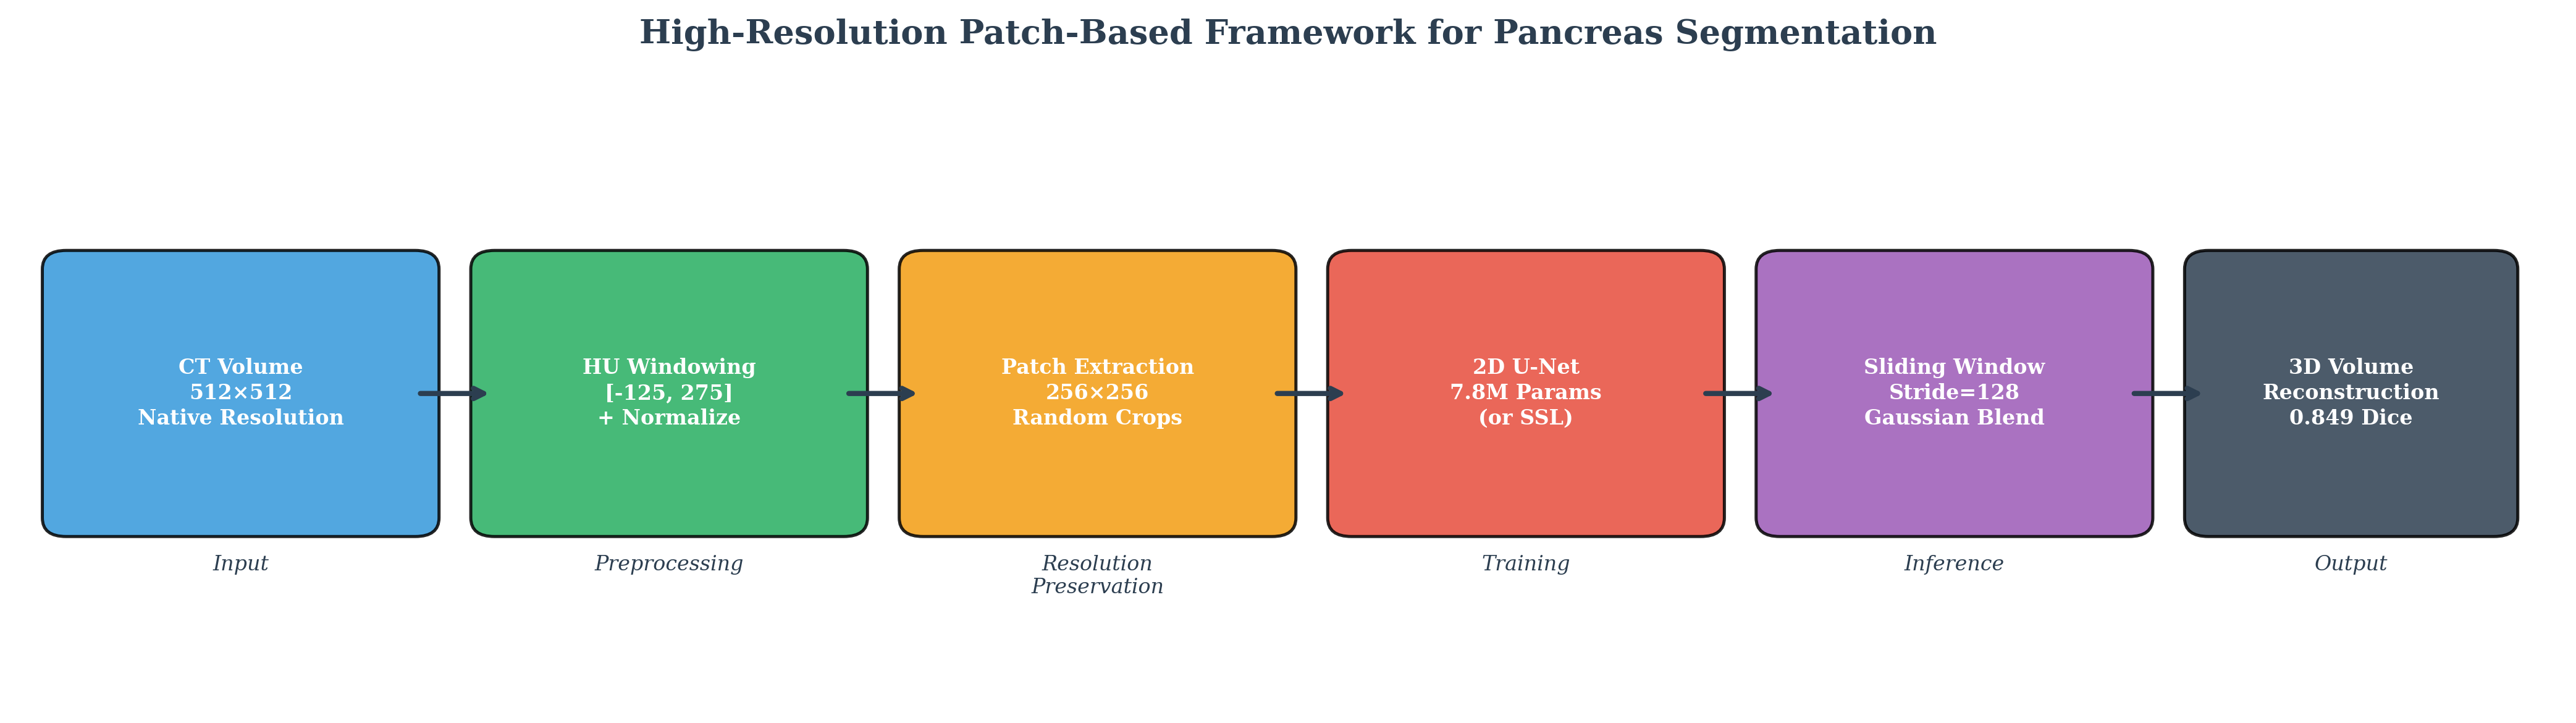
\includegraphics[width=0.95\textwidth]{pipeline_overview.png}
\caption{Overview of the proposed high-resolution patch-based framework. Native $512 \times 512$ CT slices undergo domain-specific HU windowing, followed by $256 \times 256$ patch extraction that preserves the original voxel resolution. A lightweight 2D U-Net (7.8M parameters) is trained on these patches. During inference, a sliding window with Gaussian blending reconstructs the full-resolution prediction, which is aggregated into a 3D segmentation volume.}
\label{fig:pipeline_overview}
\end{figure*}

\subsection{Data and Preprocessing}
We utilized the public Medical Segmentation Decathlon (MSD) Task07\_Pancreas dataset, consisting of 282 contrast-enhanced portal venous phase abdominal CT volumes with voxel-level annotations for both pancreatic parenchyma and tumour. Following standard practice for pancreas segmentation benchmarks, we merged the parenchyma and tumour labels into a single binary foreground class (pancreas vs.\ background). The native axial resolution is $512 \times 512$ pixels with variable slice thickness ranging from 1.0 to 2.5~mm. We partitioned the dataset into 271 volumes for training, 10 for validation, and 4 held-out test volumes (Pancreas 001, 004, 005, 006) for final 3D volumetric evaluation. After extracting 2D axial slices containing pancreatic tissue, the training set yielded 9,798 image-mask pairs.

For cross-dataset evaluation, we additionally acquired the external TCIA Pancreas-CT dataset ($N=80$) \cite{tcia}, collected at a different clinical site using different scanner protocols.

\subsubsection{Domain-Specific HU Windowing}
Standard abdominal windowing clips HU values to $[-100, 240]$. However, the pancreas often exhibits subtle intensity gradients that blend into surrounding fat and vascular structures at the boundaries of this range. We empirically identified and applied an optimized window of $[-125, 275]$, which better captures the low-contrast pancreatic boundaries. The clipped values were subsequently min-max normalized to $[0, 1]$.

\subsubsection{Resolution Preservation Strategy}
Instead of downsampling the native $512 \times 512$ axial slices, we employed a patch-based extraction strategy. During training, $256 \times 256$ patches were randomly cropped from the native resolution slices, serving simultaneously as a data augmentation mechanism through spatial jittering. This approach preserves the original voxel spacing ($\sim$0.7~mm $\times$ 0.7~mm) and allows the network to learn from uncompromised pixel data while maintaining manageable GPU memory footprints. During inference, a sliding-window approach with a stride of 128 pixels was used to reconstruct the full $512 \times 512$ probability map, with Gaussian weighting applied to smooth overlapping predictions at patch boundaries.

\subsubsection{Semi-Supervised Data Splits}
For semi-supervised experiments, we fixed the validation and test sets and partitioned the 271-volume training pool into labeled and unlabeled subsets at three ratios. The 10\% split used 27 labeled and 244 unlabeled volumes; the 25\% split used 67 labeled and 204 unlabeled volumes; and the 50\% split used 135 labeled and 136 unlabeled volumes. Splits were nested (i.e., the 10\% labeled set is a subset of the 25\% set, which is a subset of the 50\% set) to ensure fair and monotonic comparison across data regimes.

\subsection{Network Architecture}
Our baseline framework employs a standard 2D U-Net \cite{unet} architecture adapted for high-resolution patch-based segmentation (Fig.~\ref{fig:architecture}). The encoder consists of four downsampling levels, each featuring two consecutive $3 \times 3$ convolutional layers with Rectified Linear Unit (ReLU) activation, followed by a $2 \times 2$ max-pooling operation. The number of feature channels doubles at each level, progressing from 32 to 64, 128, 256, and 512 at the bottleneck. The total encoder-decoder network comprises approximately 7.8M trainable parameters.

The decoder pathway mirrors the encoder, utilizing $2 \times 2$ transposed convolutions for upsampling. Skip connections concatenate the corresponding encoder feature maps with the upsampled decoder maps to recover fine spatial details lost during pooling. The final layer is a $1 \times 1$ convolution with a sigmoid activation function, producing a pixel-wise probability map for the pancreatic tissue.

\begin{figure*}[!htbp]
\centering
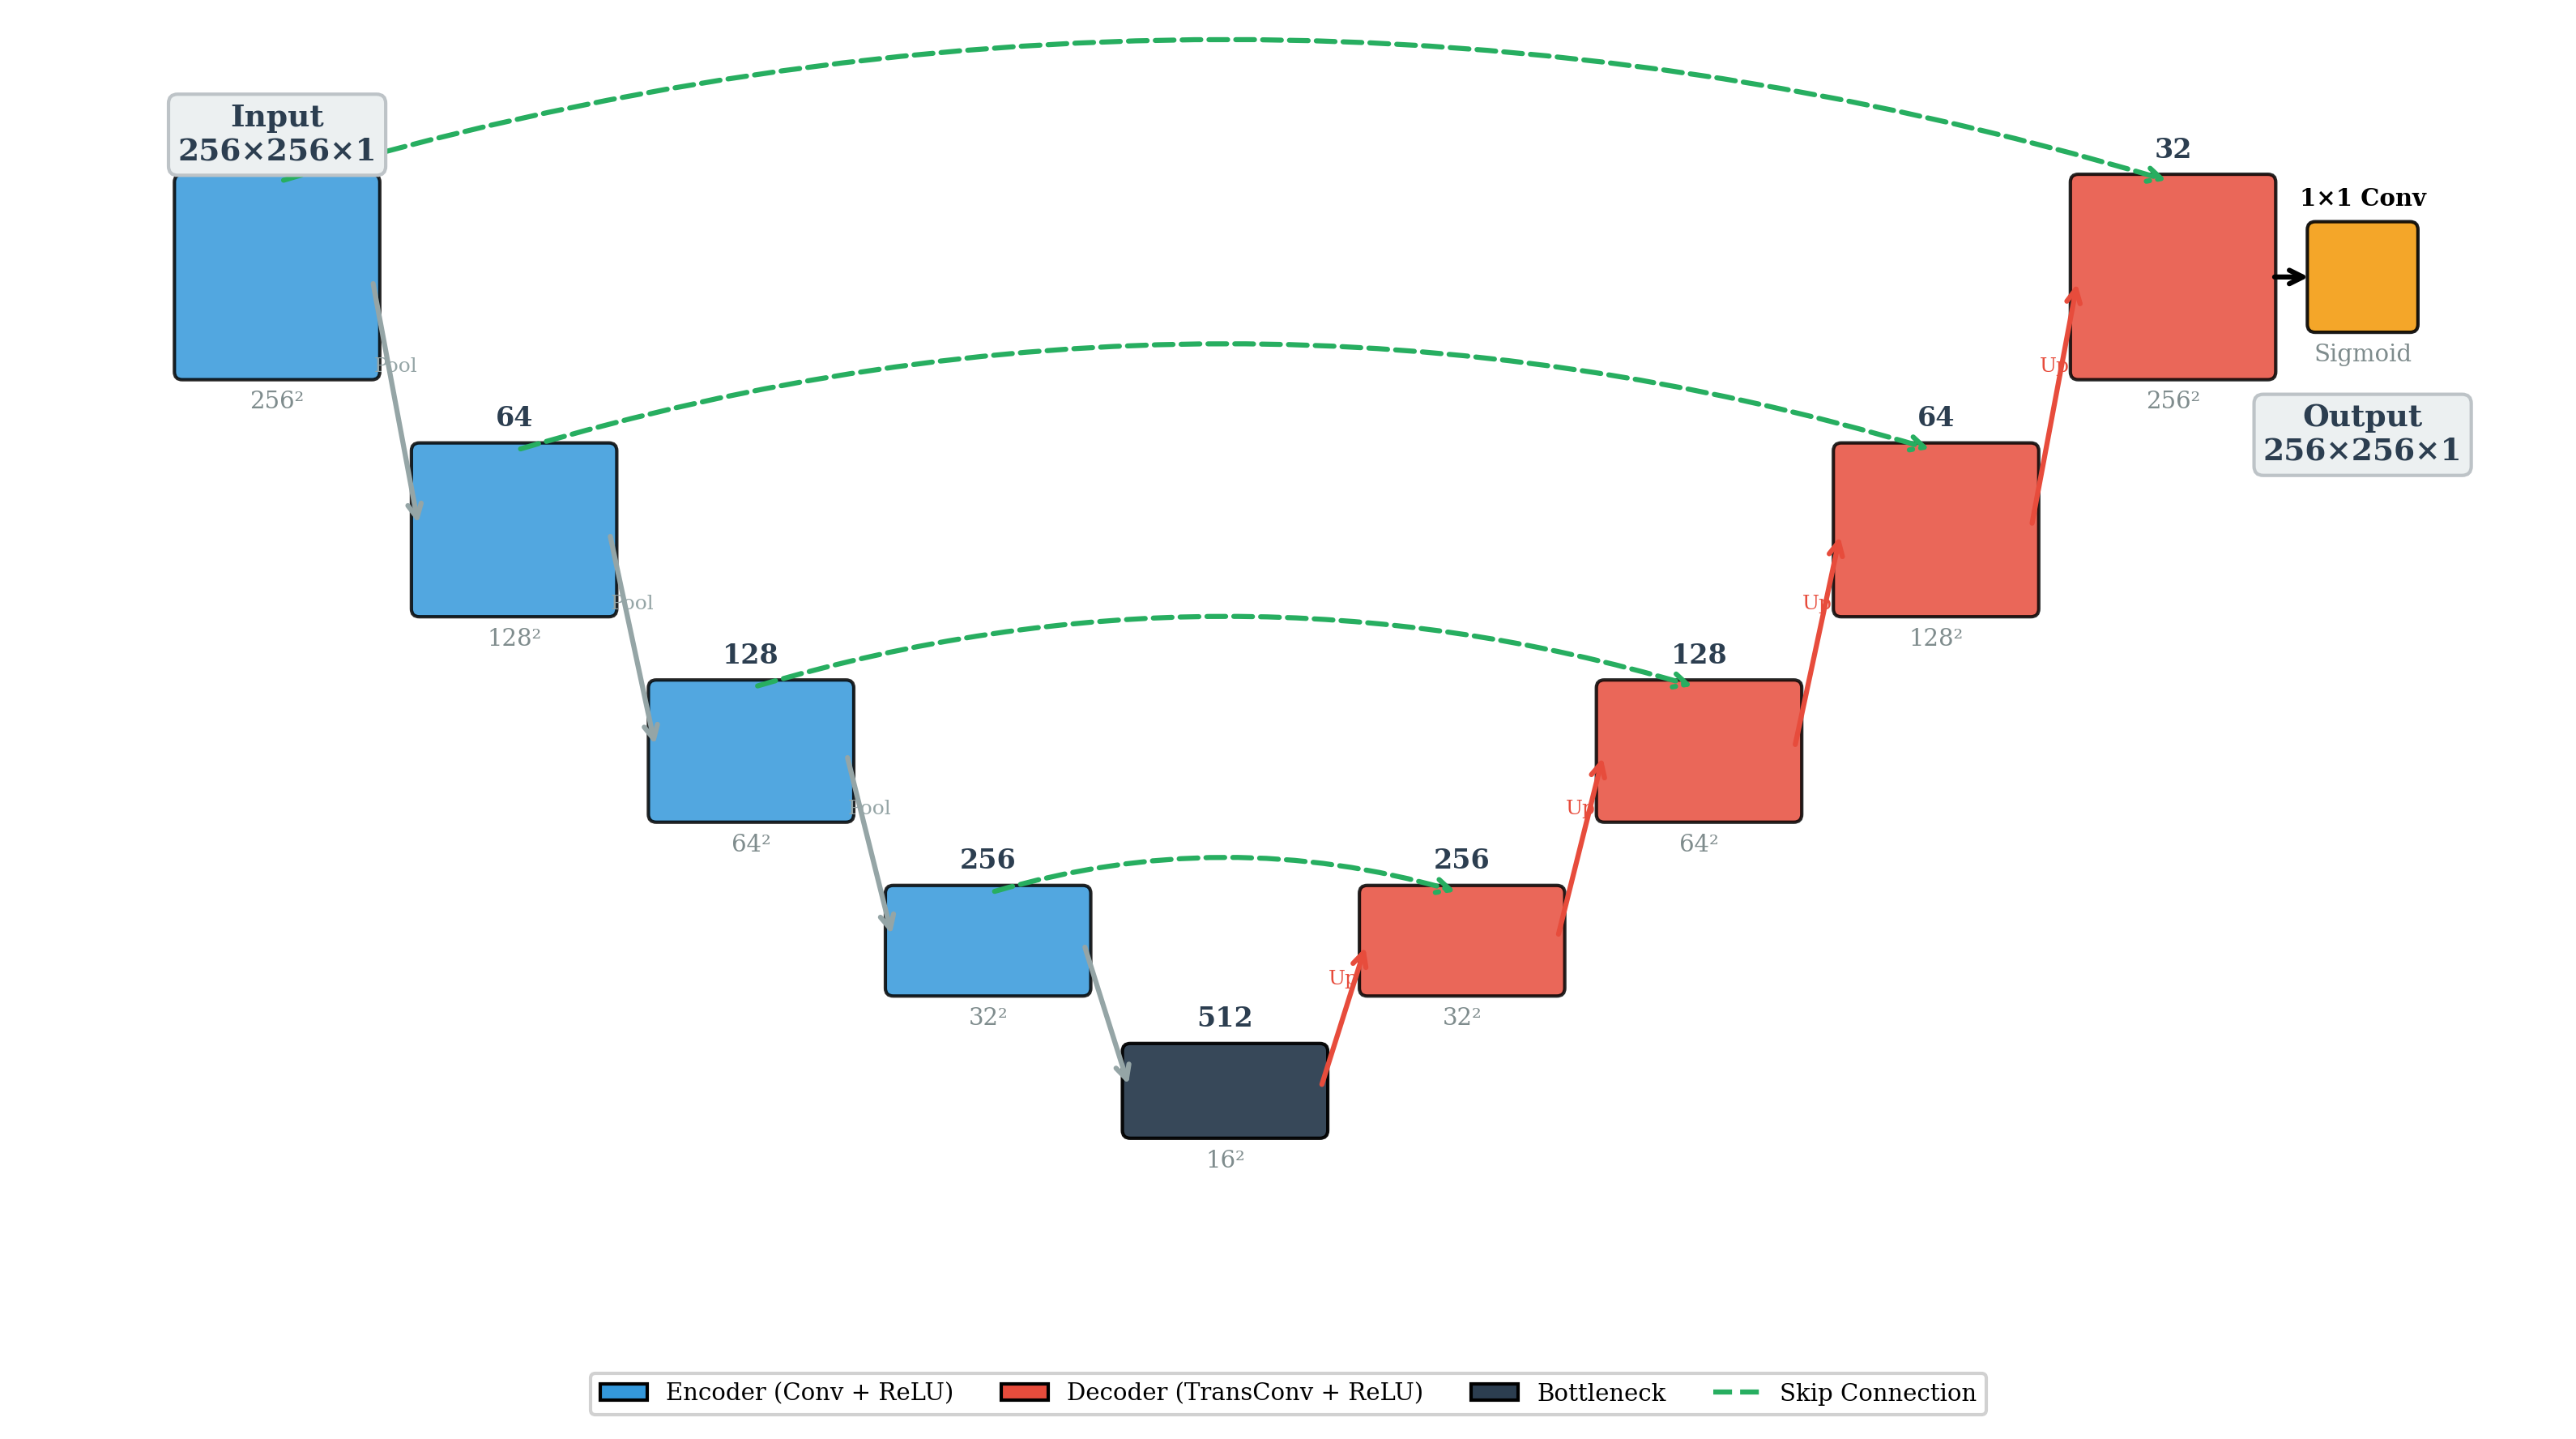
\includegraphics[width=0.95\textwidth]{architecture_unet.png}
\caption{Architecture of the proposed high-resolution patch-based U-Net. The encoder (blue) progressively downsamples from $256^2$ to $16^2$ while increasing feature channels from 32 to 512. The decoder (red) mirrors this path with transposed convolutions. Skip connections (dashed) concatenate encoder features with decoder maps to recover spatial detail. Total parameters: $\sim$7.8M.}
\label{fig:architecture}
\end{figure*}

\subsection{Architectural Baselines}
To isolate the effect of resolution versus architecture, we evaluated the following five configurations:
\begin{enumerate}
    \item \textbf{Patch-based SOTA (Our Method):} A standard 4-level U-Net ($\sim$7.8M params) trained on native-resolution $256 \times 256$ patches.
    \item \textbf{Ablation 256$\times$256:} The same U-Net architecture trained on full CT slices globally downsampled to $256 \times 256$.
    \item \textbf{Ablation 128$\times$128:} The same U-Net architecture trained on full CT slices globally downsampled to $128 \times 128$.
    \item \textbf{Transformer Baseline:} A Vision Transformer U-Net (TransUNet style) \cite{transunet} trained on the native patches to evaluate the necessity of complex self-attention mechanisms.
    \item \textbf{nnU-Net Baseline:} The self-configuring nnU-Net framework \cite{nnunet}, using its \textit{3d\_fullres} configuration trained for 1000 epochs on our dataset.
\end{enumerate}

\subsection{Semi-Supervised Learning (SSL) Framework}
To address the clinical bottleneck of voxel-level annotation, we investigated the annotation efficiency of three state-of-the-art SSL paradigms (Fig.~\ref{fig:ssl_framework}):
\begin{enumerate}
    \item \textbf{Mean Teacher (MT) \cite{tarvainen2017mean}:} A consistency-regularization approach where a student model learns from the exponential moving average (EMA) of its own weights (the teacher). MSE consistency is enforced between their predictions on unlabeled data.
    \item \textbf{Uncertainty-Aware Mean Teacher (UA-MT) \cite{uamt}:} An extension of MT that utilizes Monte Carlo (MC) Dropout to estimate the teacher's epistemic uncertainty. The student learns only from regions where the teacher is highly confident, which is particularly important for the ambiguous boundaries of the pancreas.
    \item \textbf{Cross-Pseudo Supervision (CPS) \cite{cps}:} A mutual-learning approach where two identically structured networks with different random initializations generate pseudo-labels to supervise each other.
\end{enumerate}

\begin{figure*}[!htbp]
\centering
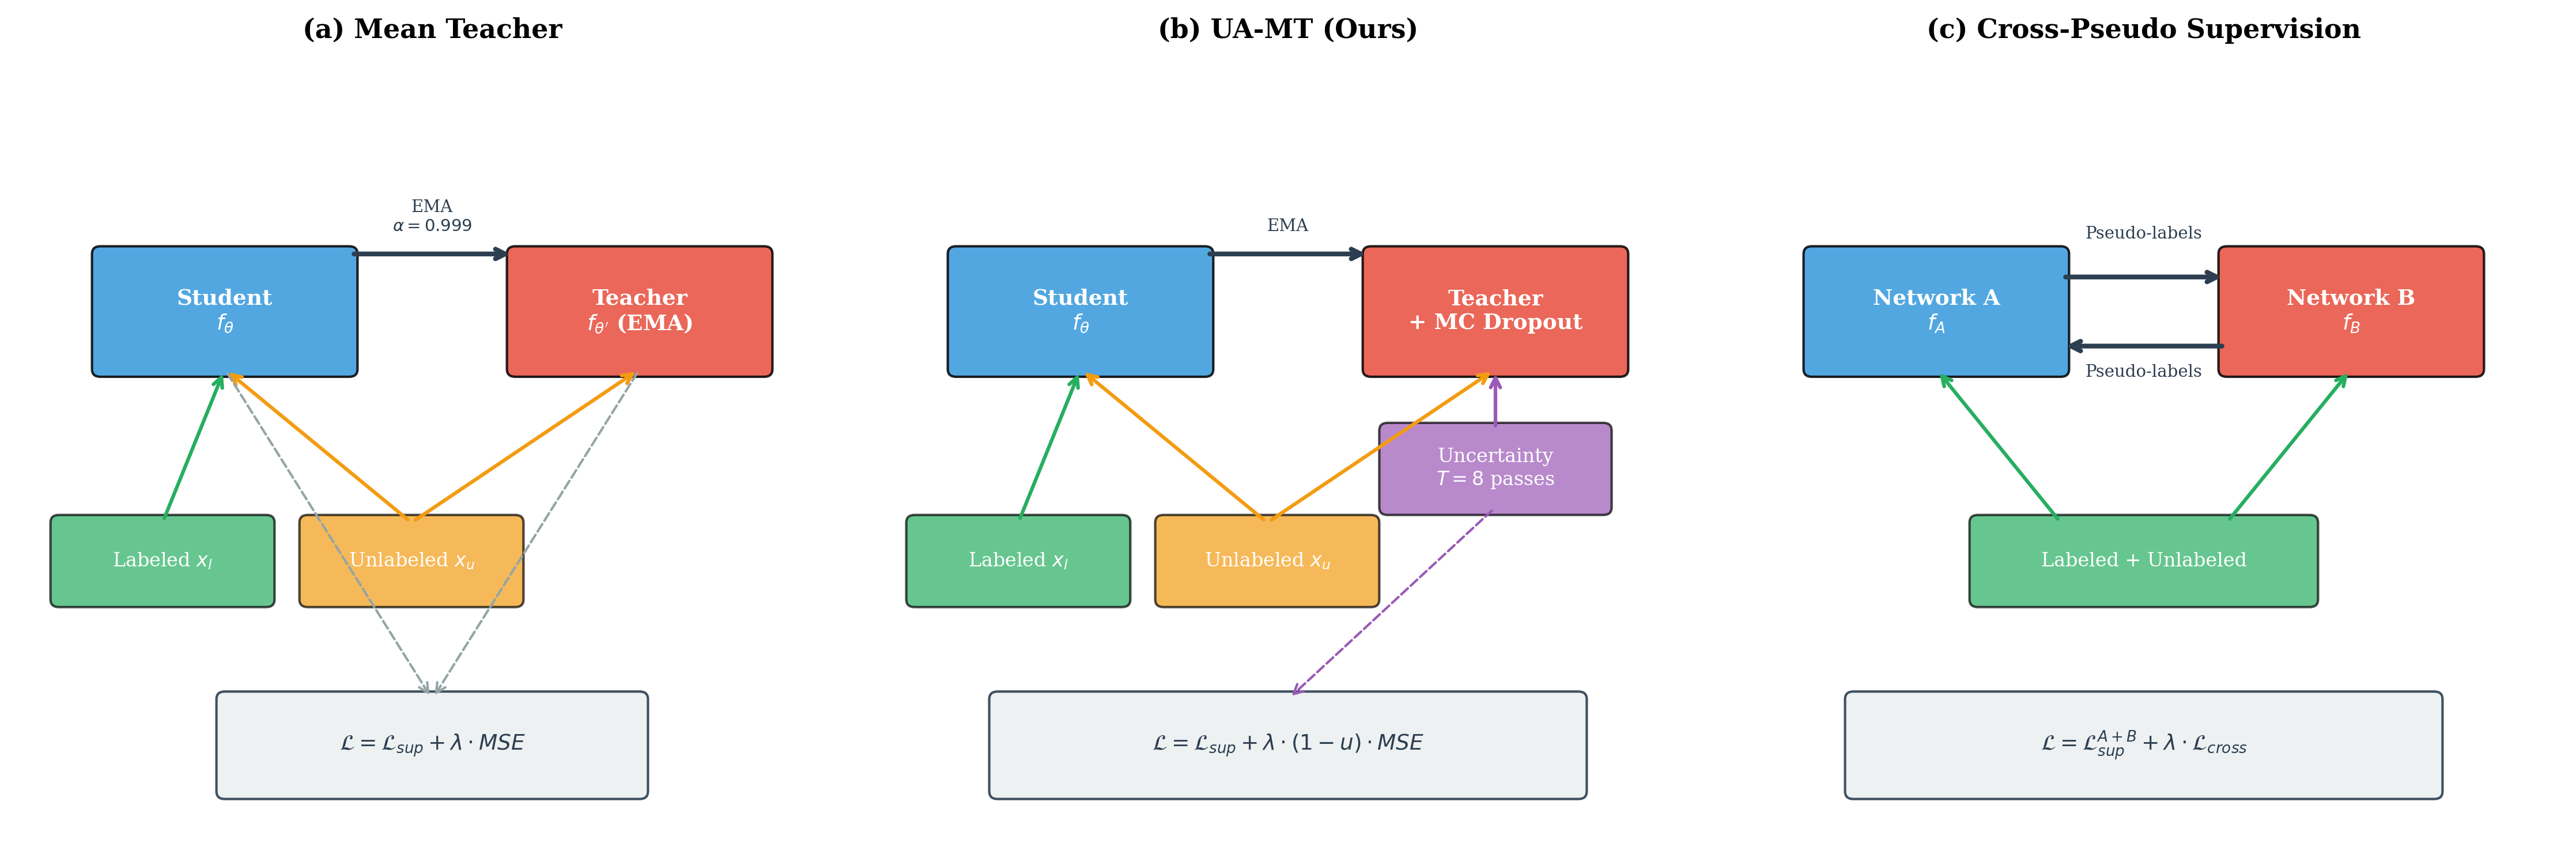
\includegraphics[width=0.95\textwidth]{ssl_framework_overview.png}
\caption{Overview of the three semi-supervised learning frameworks. (a)~Mean Teacher enforces MSE consistency between student and EMA teacher predictions on unlabeled data. (b)~UA-MT extends the Mean Teacher with Monte Carlo Dropout uncertainty estimation ($T=8$ passes), weighting the consistency loss by teacher confidence $(1-u)$ to suppress learning from ambiguous regions. (c)~Cross-Pseudo Supervision trains two independently initialized networks that mutually generate pseudo-labels.}
\label{fig:ssl_framework}
\end{figure*}

\subsection{Loss Formulation}
\subsubsection{Supervised Loss}
For fully supervised training, we used the binary cross-entropy (BCE) loss:
\begin{equation}
\mathcal{L}_{\text{sup}} = -\frac{1}{N}\sum_{i=1}^{N}\left[y_i \log(\hat{y}_i) + (1-y_i)\log(1-\hat{y}_i)\right]
\label{eq:bce}
\end{equation}
where $y_i$ and $\hat{y}_i$ denote the ground truth and predicted probability for voxel $i$, respectively.

\subsubsection{Mean Teacher Consistency Loss}
The total loss for the Mean Teacher framework combines the supervised loss on labeled data with an MSE consistency term on unlabeled data:
\begin{equation}
\mathcal{L}_{\text{MT}} = \mathcal{L}_{\text{sup}} + \lambda(t) \cdot \frac{1}{M}\sum_{j=1}^{M}\|f_{\theta'}(x_u^j) - f_\theta(x_u^j)\|^2
\label{eq:mt}
\end{equation}
where $f_\theta$ and $f_{\theta'}$ denote the student and teacher networks, $x_l$ and $x_u$ are labeled and unlabeled inputs, and $\lambda(t)$ is a time-dependent consistency weight that follows a sigmoid ramp-up schedule over the first 40 epochs.

\subsubsection{UA-MT Uncertainty-Weighted Loss}
The UA-MT extends the Mean Teacher by weighting the consistency loss with an uncertainty mask derived from $T$ stochastic forward passes through the teacher:
\begin{equation}
u_i = -\frac{1}{T}\sum_{t=1}^{T} \hat{y}_i^{(t)} \log \hat{y}_i^{(t)}
\label{eq:uncertainty}
\end{equation}
\begin{equation}
\mathcal{L}_{\text{UA-MT}} = \mathcal{L}_{\text{sup}} + \lambda(t) \cdot \frac{1}{M}\sum_{j=1}^{M}(1 - u_j)\|f_{\theta'}(x_u^j) - f_\theta(x_u^j)\|^2
\label{eq:uamt}
\end{equation}
where $u_i \in [0, 1]$ is the voxel-wise predictive entropy (uncertainty), and $(1 - u_j)$ serves as a confidence mask that suppresses learning from uncertain regions. We used $T=8$ MC Dropout forward passes.

\subsubsection{CPS Mutual Loss}
The CPS loss combines supervised losses from both networks with cross-pseudo supervision:
\begin{multline}
\mathcal{L}_{\text{CPS}} = \mathcal{L}_{\text{sup}}^A + \mathcal{L}_{\text{sup}}^B \\
+ \lambda(t)\left[\mathcal{L}_{\text{BCE}}(\text{sg}(p_B), p_A) + \mathcal{L}_{\text{BCE}}(\text{sg}(p_A), p_B)\right]
\label{eq:cps}
\end{multline}
where $p_A$ and $p_B$ are the outputs of networks A and B, and $\text{sg}(\cdot)$ denotes the stop-gradient operator.

\subsection{Training Details}
All experiments were conducted on an NVIDIA Tesla V100 GPU (32~GB) using TensorFlow 2.x. Table~\ref{tab:hyperparams} summarizes the key hyperparameters. All models were optimized with Adam ($\text{lr} = 10^{-4}$) for 100 epochs, except nnU-Net which used its self-configured settings for 1000 epochs. The EMA decay coefficient for teacher-student frameworks was $\alpha = 0.999$. UA-MT employed dropout rate 0.1 in all convolutional blocks for MC uncertainty estimation. No additional data augmentation beyond random patch cropping was applied.

\begin{table}[!htbp]
\centering
\caption{Training Hyperparameters}
\label{tab:hyperparams}
\small
\begin{tabular}{lcccc}
\toprule
\textbf{Config.} & \textbf{Batch} & \textbf{Epochs} & \textbf{Loss} & \textbf{Params} \\
\midrule
Supervised & 32 & 100 & BCE & 7.8M \\
Ablation & 32 & 100 & BCE & 7.8M \\
ViT Baseline & 16 & 100 & BCE & $\sim$105M \\
nnU-Net & Auto & 1000 & DC+CE & $\sim$92M \\
MT (SSL) & 16 & 100 & BCE+MSE & 7.8M \\
UA-MT (SSL) & 8 & 100 & BCE+MSE & 7.8M \\
CPS (SSL) & 16 & 100 & BCE+BCE & 2$\times$7.8M \\
\bottomrule
\end{tabular}
\end{table}

\subsection{Evaluation Metrics}
We report two complementary metrics. The Dice Similarity Coefficient (DSC) measures volumetric overlap:
\begin{equation}
\text{DSC} = \frac{2|P \cap G|}{|P| + |G|}
\label{eq:dice}
\end{equation}
where $P$ and $G$ denote the predicted and ground truth segmentation masks. The Intersection over Union (IoU) is defined as:
\begin{equation}
\text{IoU} = \frac{|P \cap G|}{|P \cup G|}
\label{eq:iou}
\end{equation}
During training, we monitored 2D patch-level IoU on the validation set. For final evaluation, we report 3D volumetric Dice computed by aggregating all predicted slices into a full 3D volume and comparing against the ground truth volume.

\FloatBarrier
% =====================================================================
\section{Results and Discussion}
% =====================================================================

\subsection{The Impact of Domain-Specific Windowing}
Our initial experiments isolated the effect of HU windowing using our optimized patch-based model. Table~\ref{tab:hu_windowing} presents the per-case comparison. The standard $[-100, 240]$ window achieved an average Dice of 0.7653, while the pancreas-specific $[-125, 275]$ window improved the average to 0.8147---an absolute gain of +4.94\%. Notably, the improvement is most pronounced on the challenging Pancreas\_005 case (+15.46\% Dice), where the pancreas boundary is particularly ambiguous. This underscores the sensitivity of CNNs to input intensity distributions and validates the importance of domain-specific preprocessing. Fig.~\ref{fig:hu_windowing} visualizes the effect of windowing on a representative CT slice.

\begin{figure*}[!htbp]
\centering
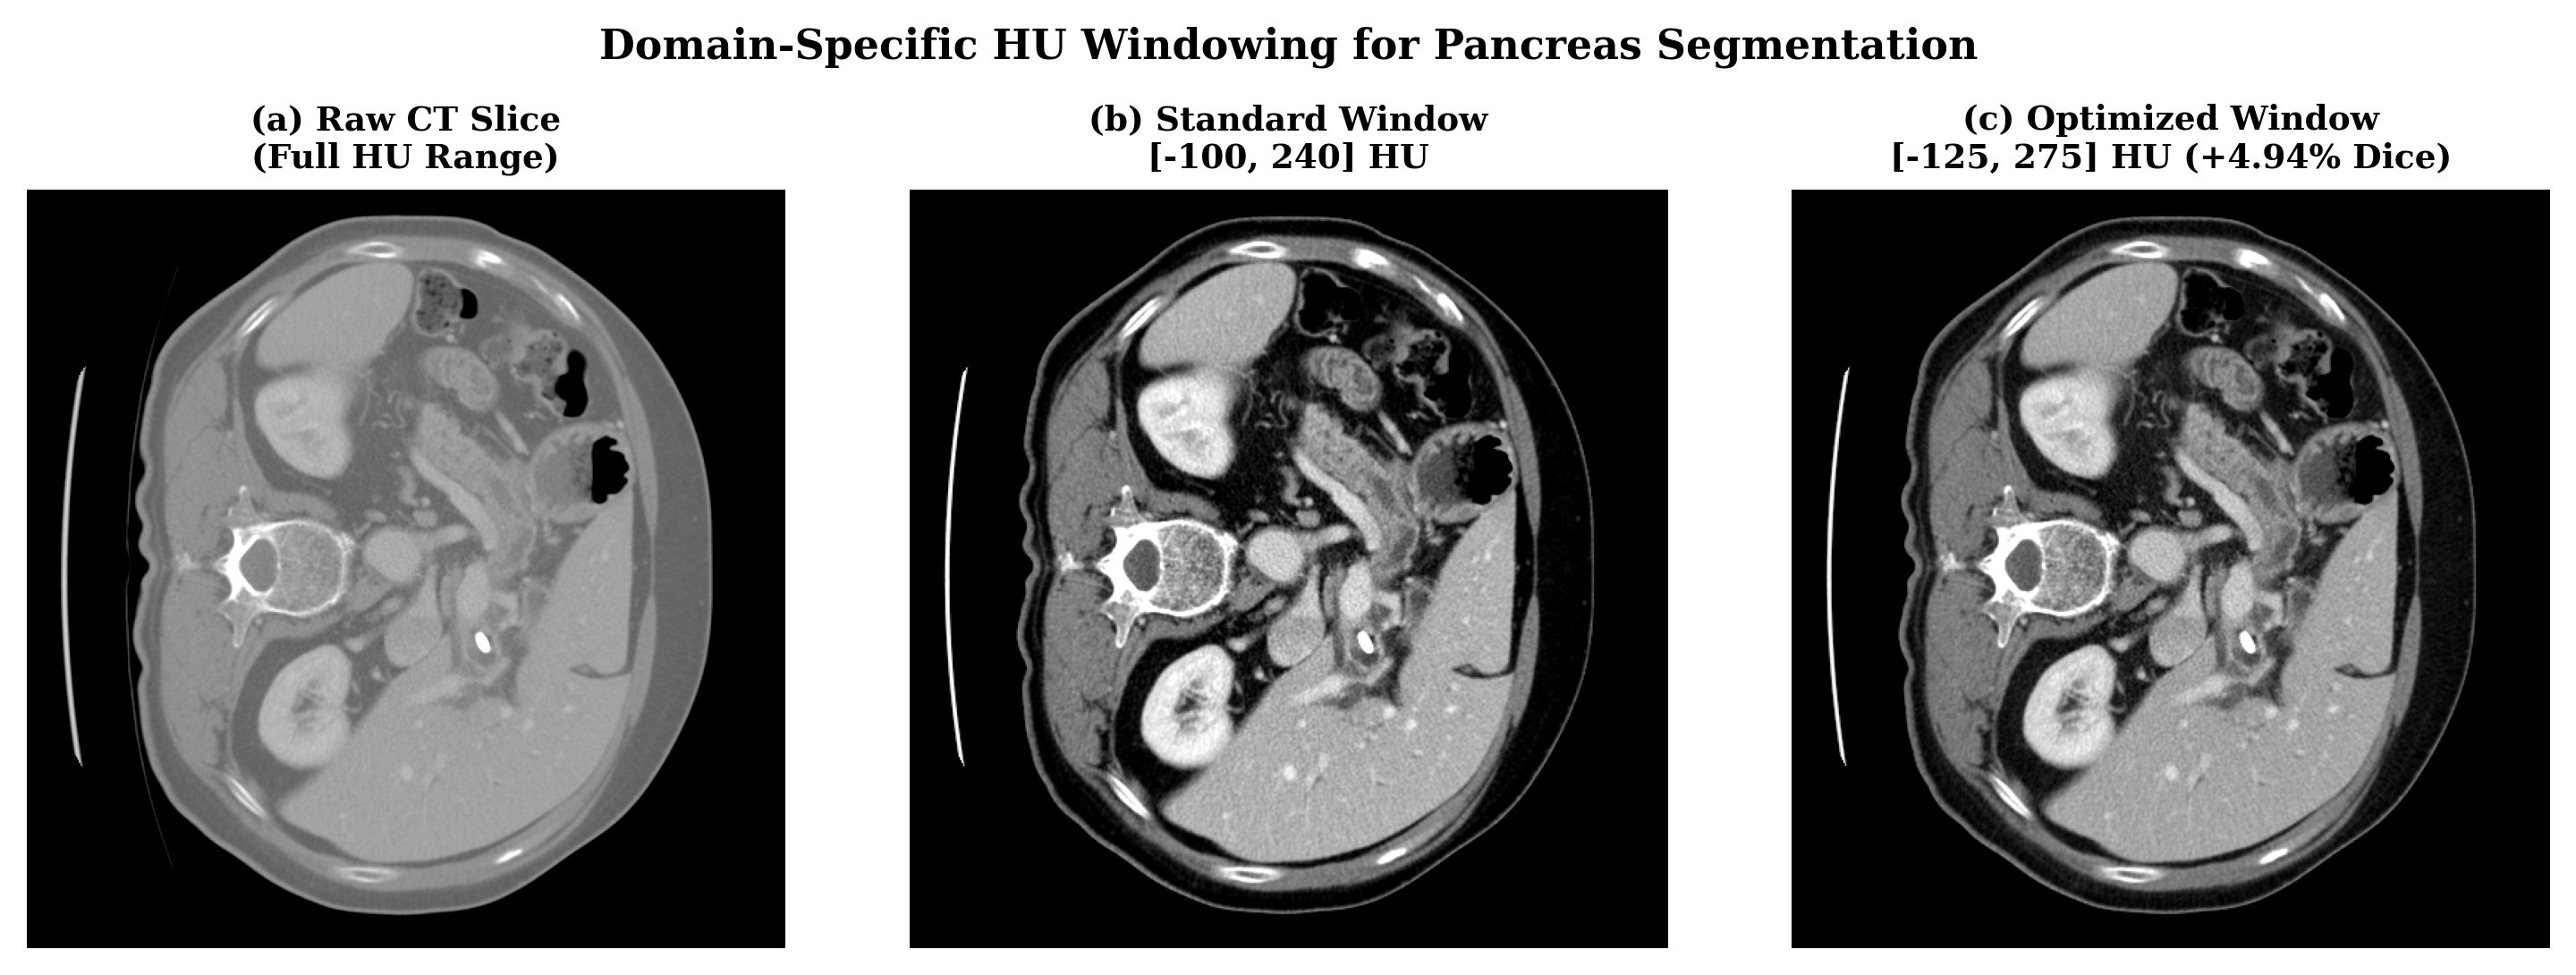
\includegraphics[width=0.95\textwidth]{hu_windowing_comparison.png}
\caption{Visual comparison of HU windowing strategies on a representative axial CT slice. (a)~Raw CT with full HU range showing low contrast. (b)~Standard abdominal window $[-100, 240]$. (c)~Our optimized pancreas-specific window $[-125, 275]$, which better preserves the subtle intensity gradients at the pancreatic boundary, contributing to a +4.94\% absolute Dice improvement.}
\label{fig:hu_windowing}
\end{figure*}

\begin{table}[!htbp]
\centering
\caption{Impact of HU Windowing on 3D Dice (Per-Case Breakdown)}
\label{tab:hu_windowing}
\small
\begin{tabular}{lccccc}
\toprule
\textbf{Window} & \textbf{001} & \textbf{004} & \textbf{005} & \textbf{006} & \textbf{Mean} \\
\midrule
Std. [-100, 240] & .910 & .824 & .542 & .786 & .765 \\
Opt. [-125, 275] & .902 & .845 & \textbf{.696} & .816 & \textbf{.815} \\
\midrule
$\Delta$ & -.008 & +.021 & \textbf{+.155} & +.030 & \textbf{+.049} \\
\bottomrule
\end{tabular}
\end{table}

\subsection{Resolution Ablation: The Collapse of the Pancreas}
We conducted a rigorous ablation study to quantify the cost of downsampling. The $128 \times 128$ full-slice model converged rapidly but stagnated at a validation IoU of 0.3036. The $256 \times 256$ full-slice model showed only a marginal improvement, reaching a validation IoU of 0.3113.

Crucially, both downsampled models dramatically underperformed our patch-based SOTA model ($0.809 \pm 0.015$ Dice, $\sim$0.69 IoU). This massive performance cliff---over 55\% relative IoU degradation---indicates that the pancreas is effectively ``lost'' to the network when native resolution is compromised. The global context provided by seeing the entire abdomen in the downsampled slices could not compensate for the loss of local boundary texture at the sub-millimeter level. The individual training dynamics for each ablation model are shown in Fig.~\ref{fig:ablation_curves}, and the comparative overview is presented in Fig.~\ref{fig:ablation_comparison}.

\begin{figure}[!htbp]
\centering
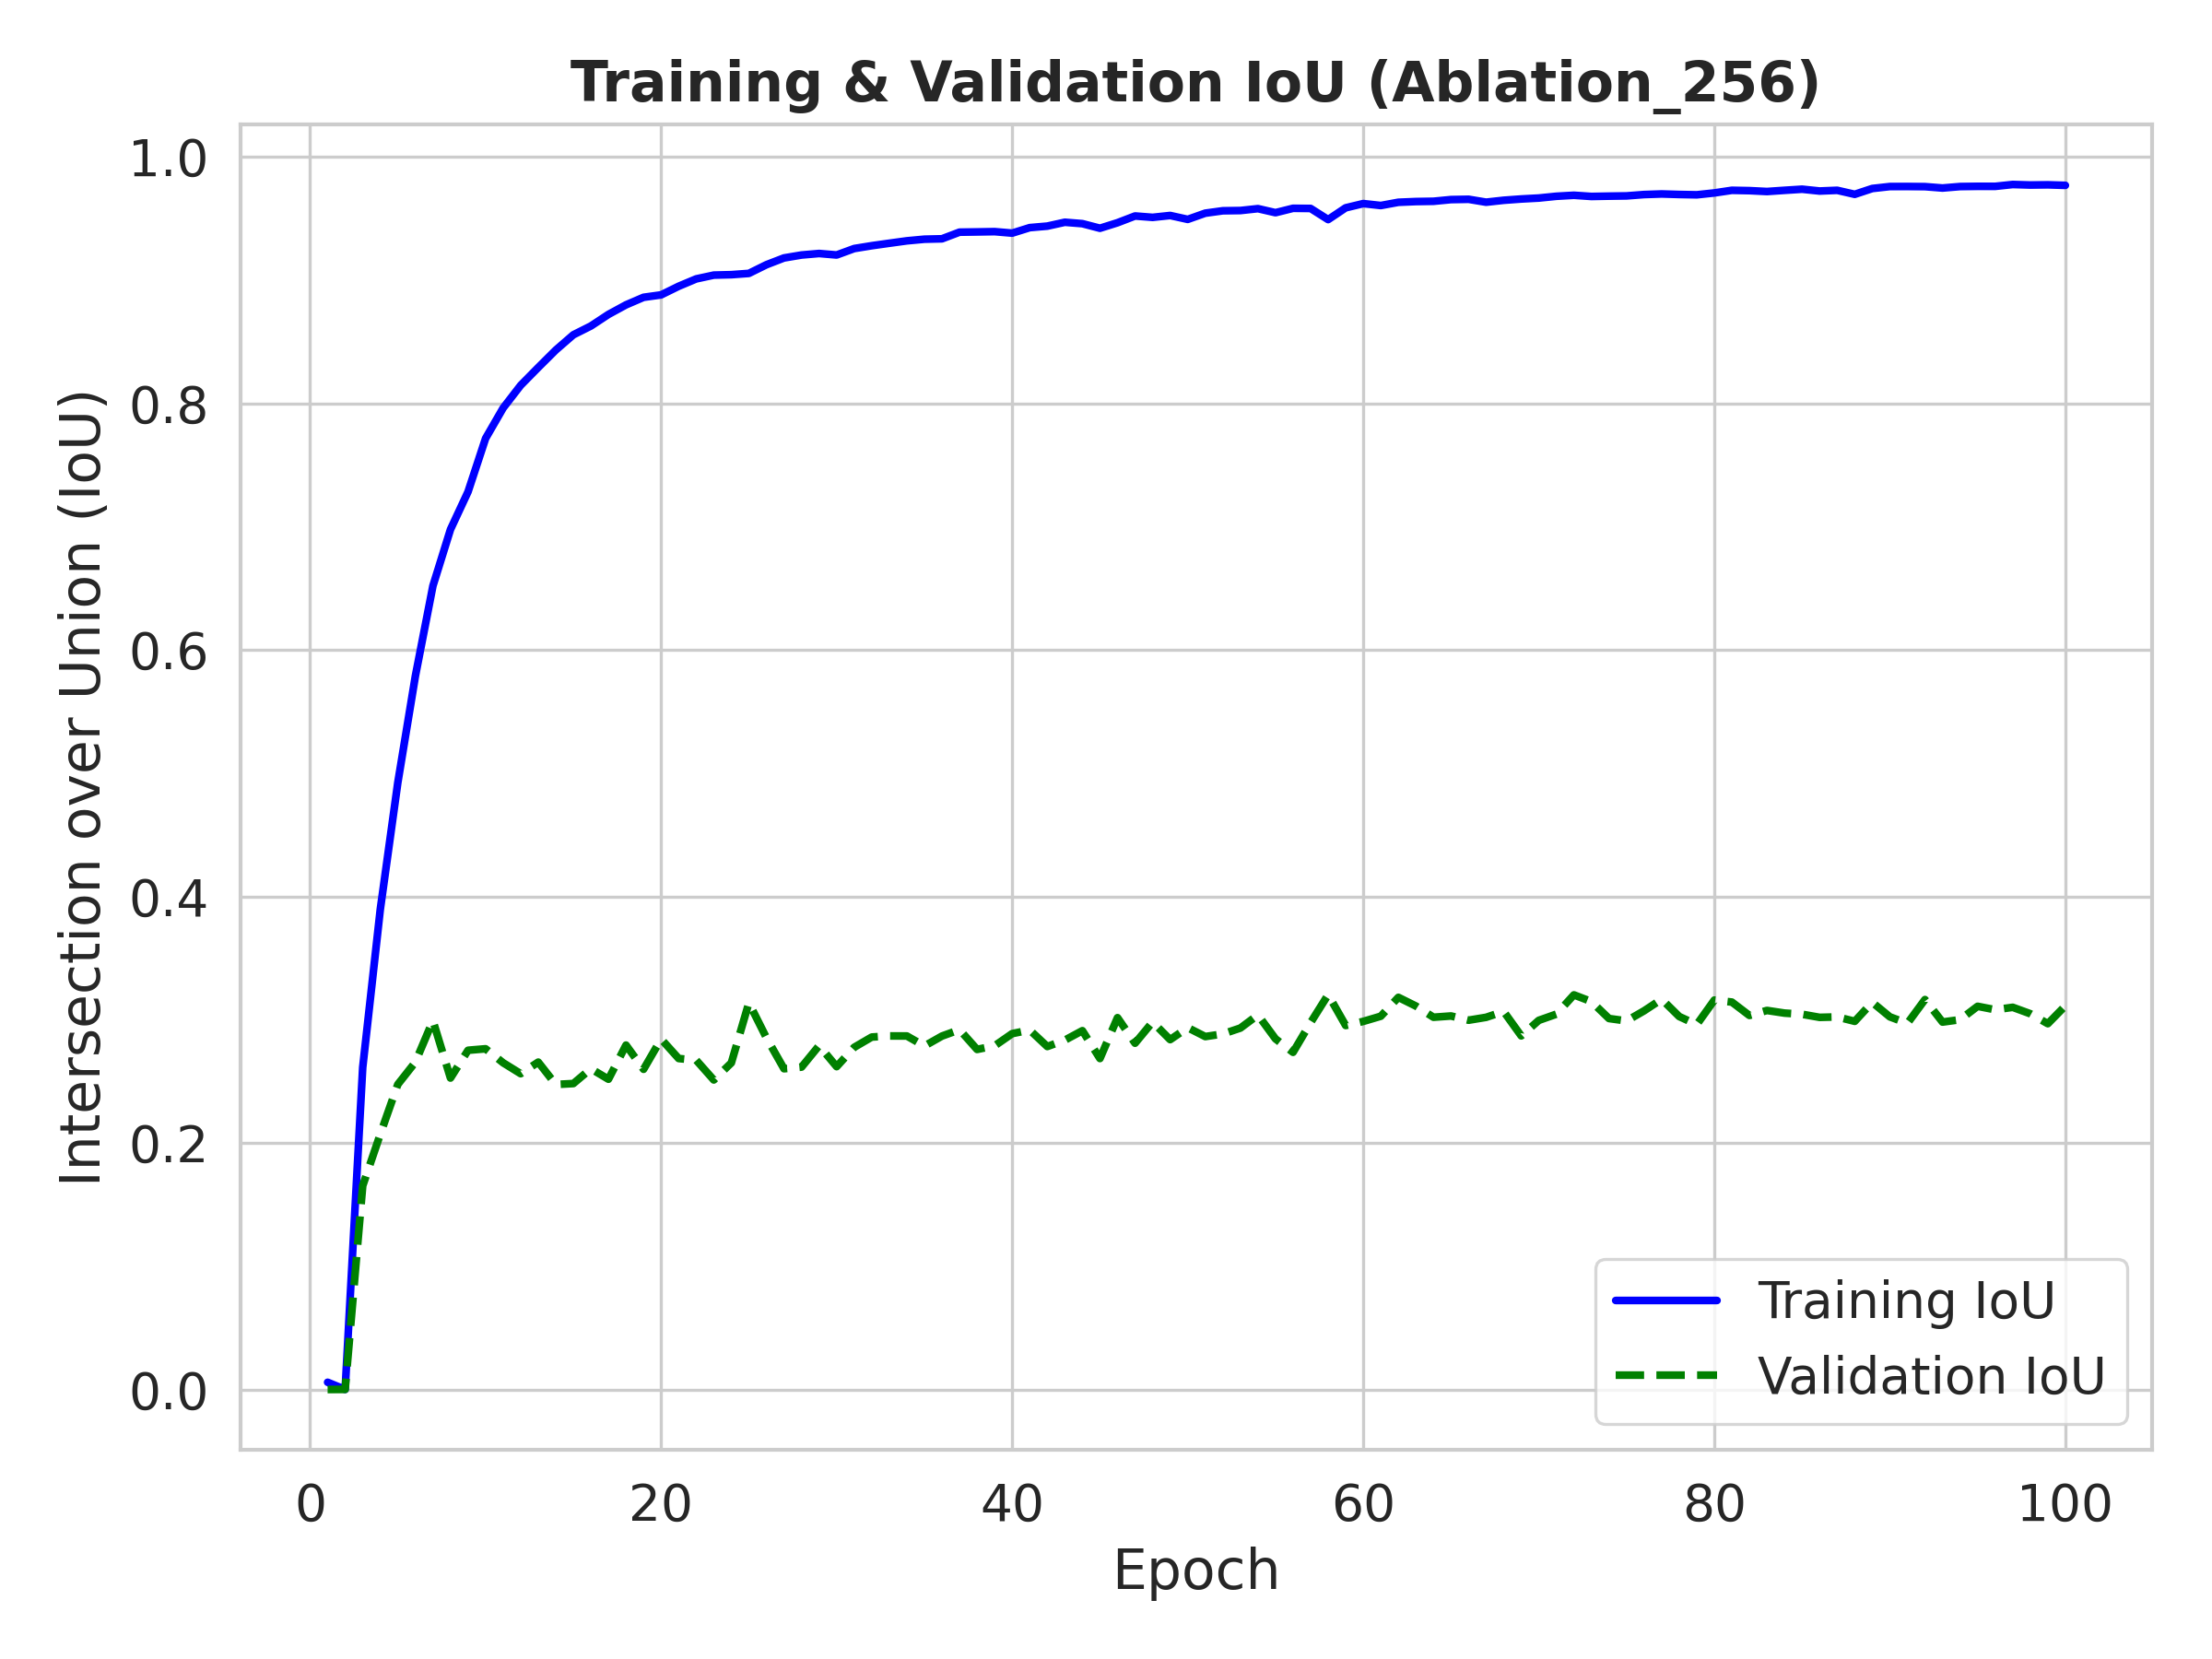
\includegraphics[width=0.49\columnwidth]{Ablation_256_iou_curve.png}
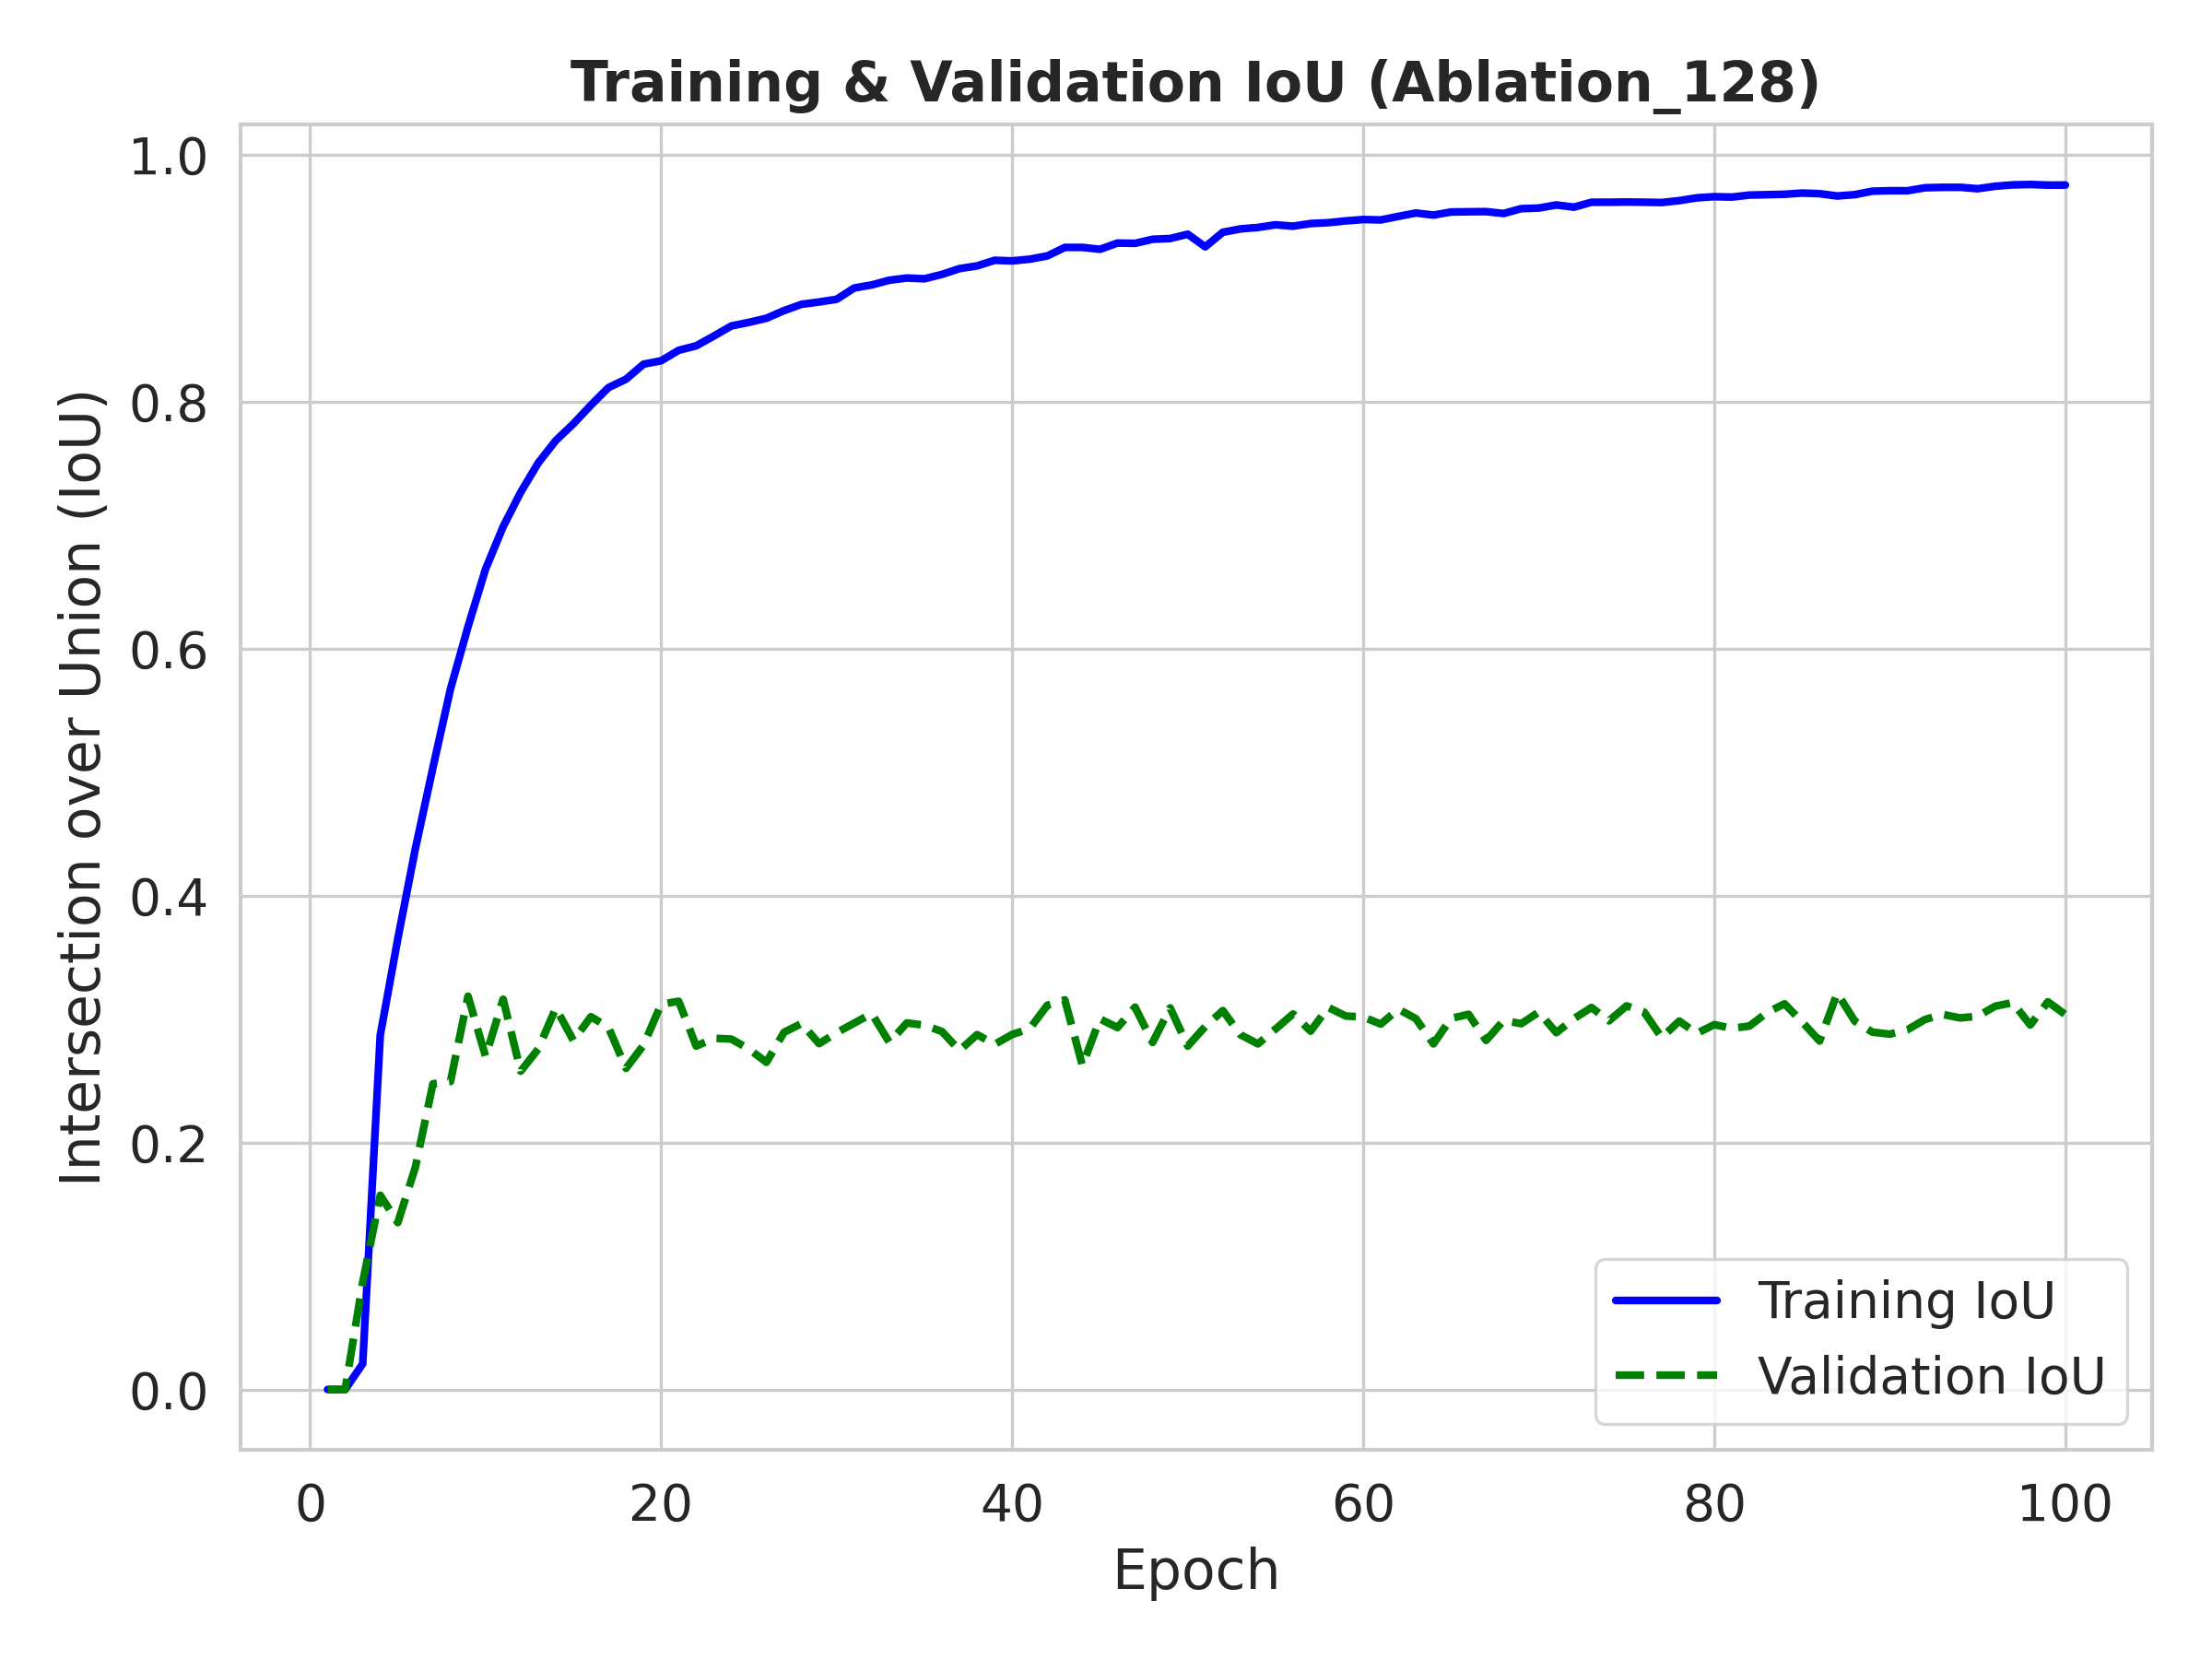
\includegraphics[width=0.49\columnwidth]{Ablation_128_iou_curve.png}
\caption{Individual validation IoU curves for the $256 \times 256$ (left) and $128 \times 128$ (right) downsampled ablation models. Both converge rapidly to low IoU values ($\sim$0.31), confirming that the resolution loss is a fundamental information bottleneck.}
\label{fig:ablation_curves}
\end{figure}

\begin{figure}[!htbp]
\centering
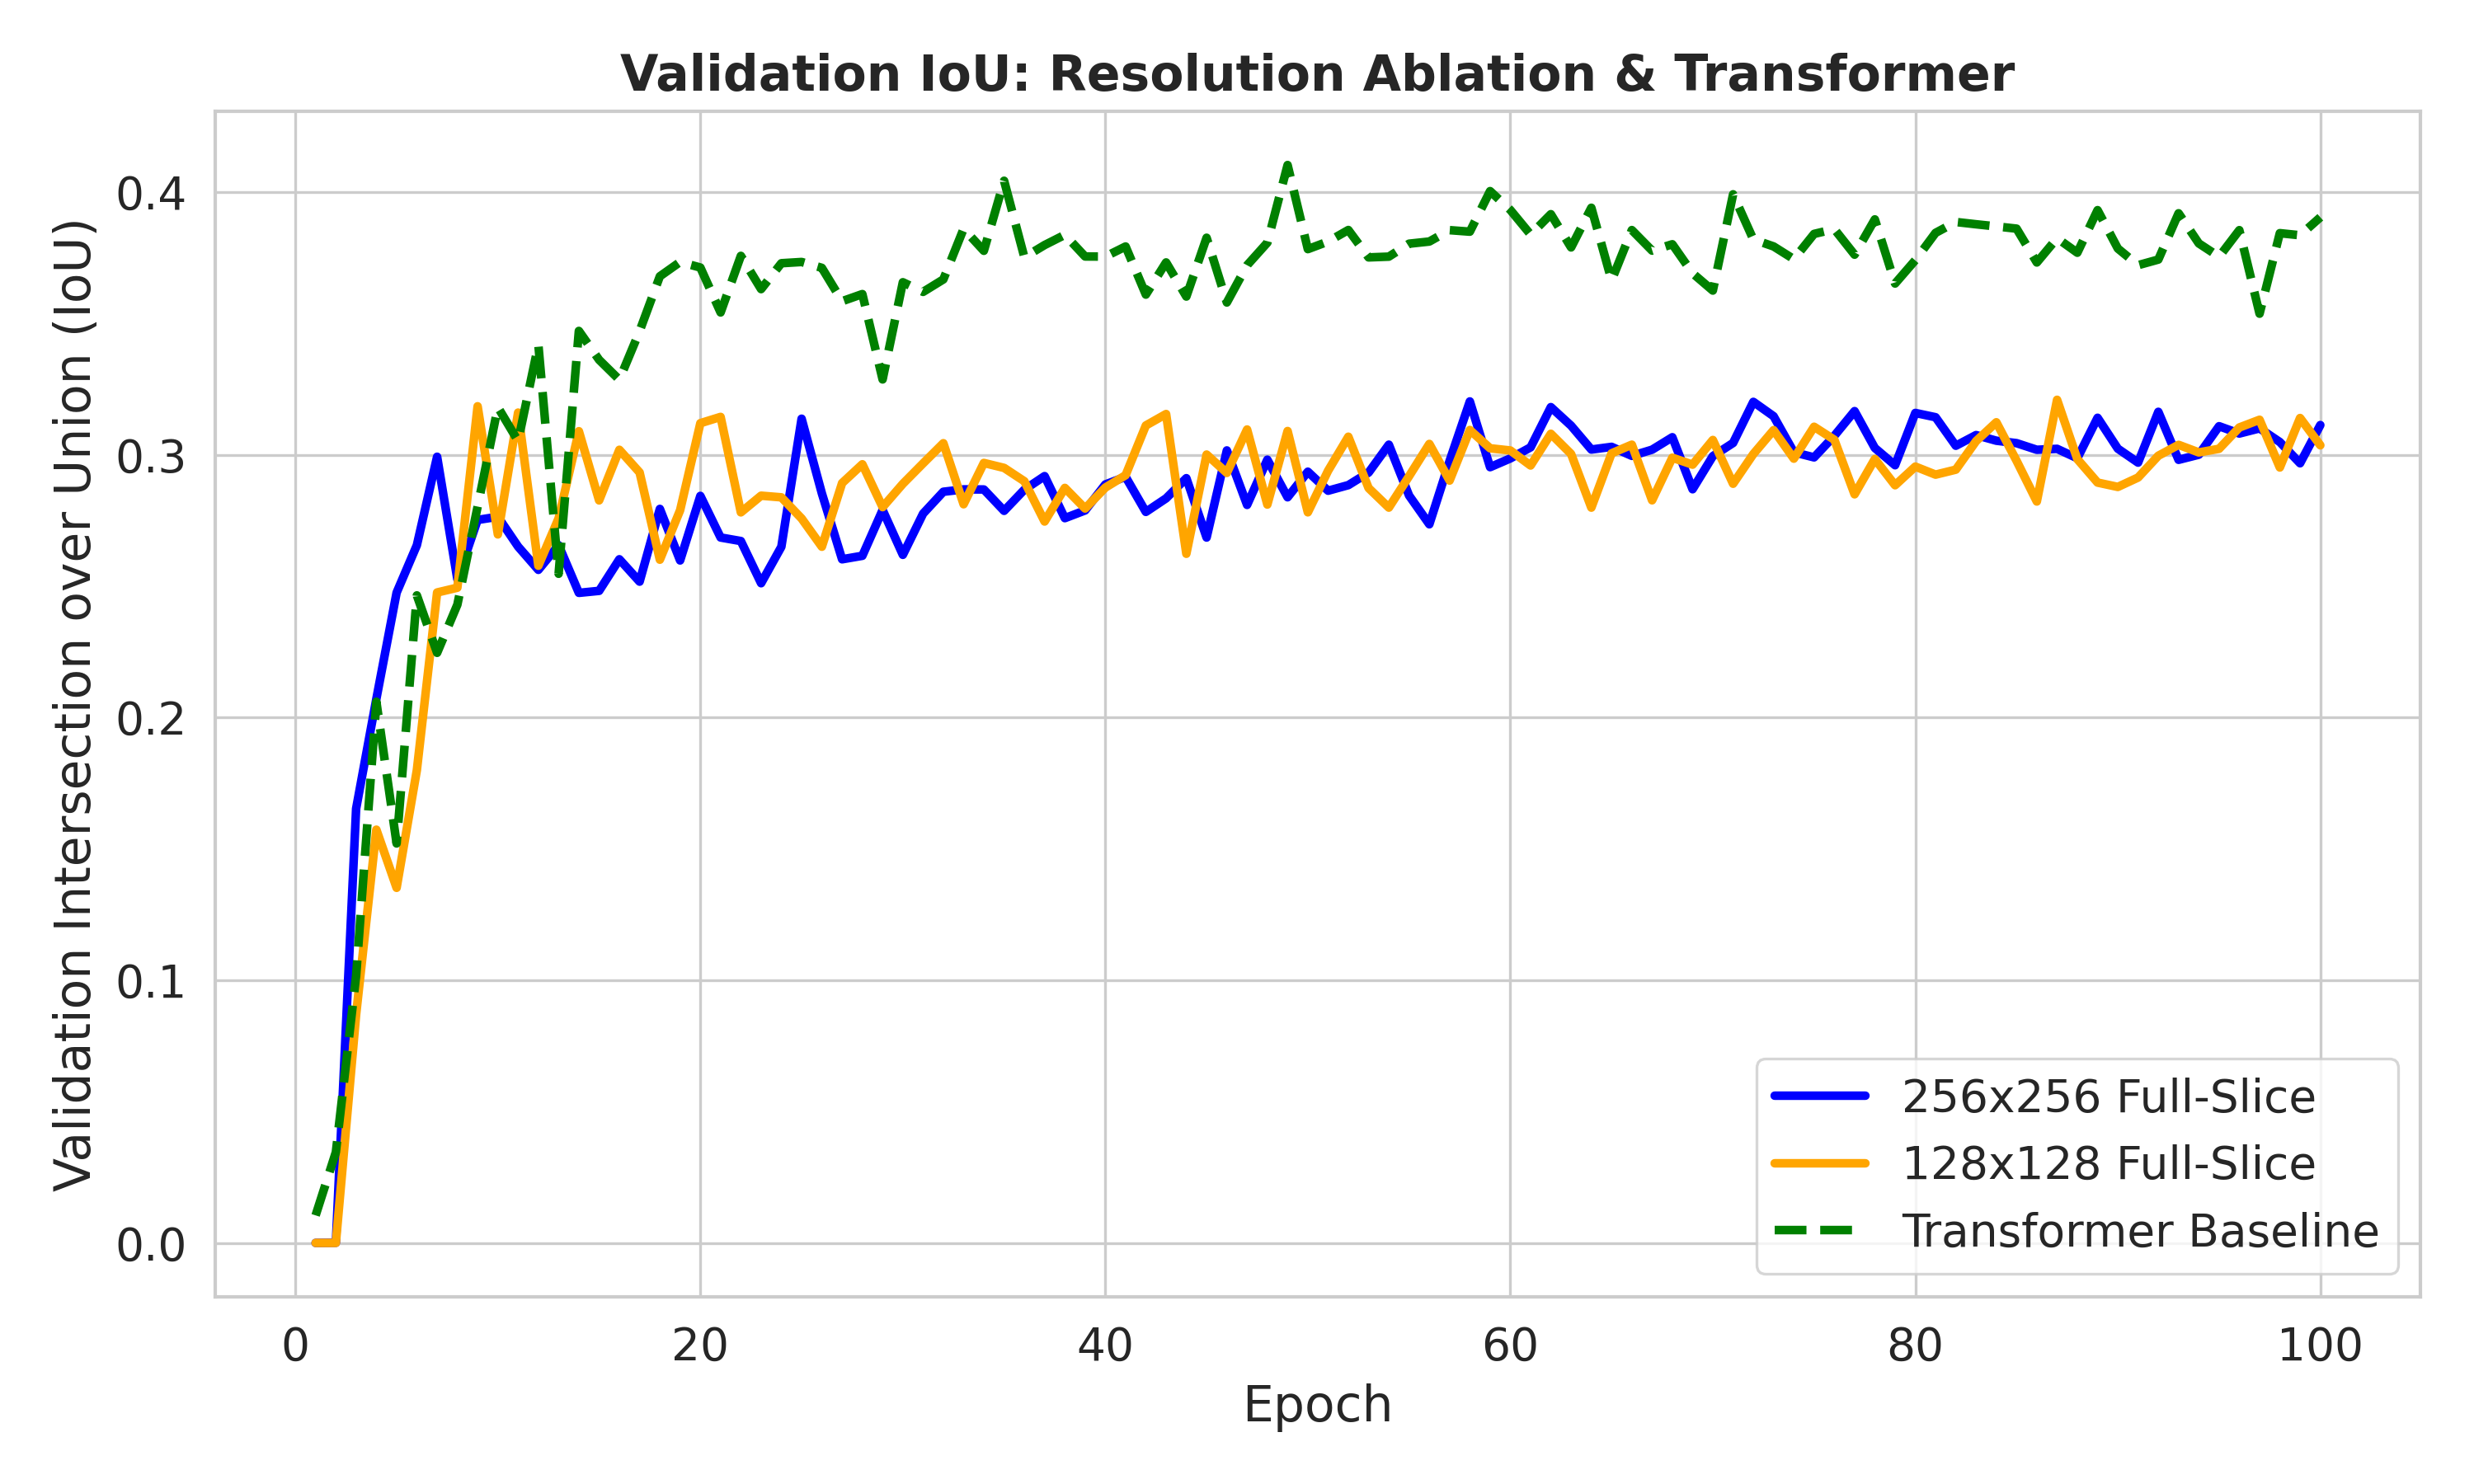
\includegraphics[width=\columnwidth]{ablation_iou_comparison.png}
\caption{Validation IoU curves for the resolution ablation study. The $128 \times 128$ and $256 \times 256$ downsampled models plateau at $\sim$0.31 IoU, while the native-resolution patch-based model achieves $\sim$0.69 IoU---a catastrophic gap that underscores the primacy of spatial fidelity for small-organ segmentation.}
\label{fig:ablation_comparison}
\end{figure}

\subsection{Frequency-Domain Analysis of Resolution Loss}
To provide theoretical grounding for the empirical results above, we analyzed the spatial frequency content of CT slices at different resolutions using 2D Fourier Transform analysis. Downsampling from native resolution to $256 \times 256$ or $128 \times 128$ acts as a low-pass filter, irreversibly destroying high-frequency components that encode fine structural details such as organ boundaries and tissue texture.

Fig.~\ref{fig:fourier_spectrum} presents the radial power spectrum comparison. The native-resolution signal (blue) retains significantly more energy at high spatial frequencies compared to the downsampled versions. Critically, the pancreas boundary frequency content (purple shaded region) overlaps substantially with the frequency bands that are attenuated or eliminated by downsampling. This explains why the segmentation performance collapses: the network cannot delineate boundaries whose spatial frequency information has been destroyed before the data reaches the model.

We further quantified this effect through Sobel edge analysis at the pancreas boundary (Fig.~\ref{fig:fourier_visual}). The mean boundary edge strength decreases from 0.436 at native resolution to 0.345 at $256 \times 256$ ($-$21\%) and 0.269 at $128 \times 128$ ($-$38\%). This progressive degradation of boundary contrast directly explains the catastrophic IoU collapse observed in our ablation study: the pancreas boundary becomes indistinguishable from surrounding tissue at reduced resolutions.

\begin{figure*}[!htbp]
\centering
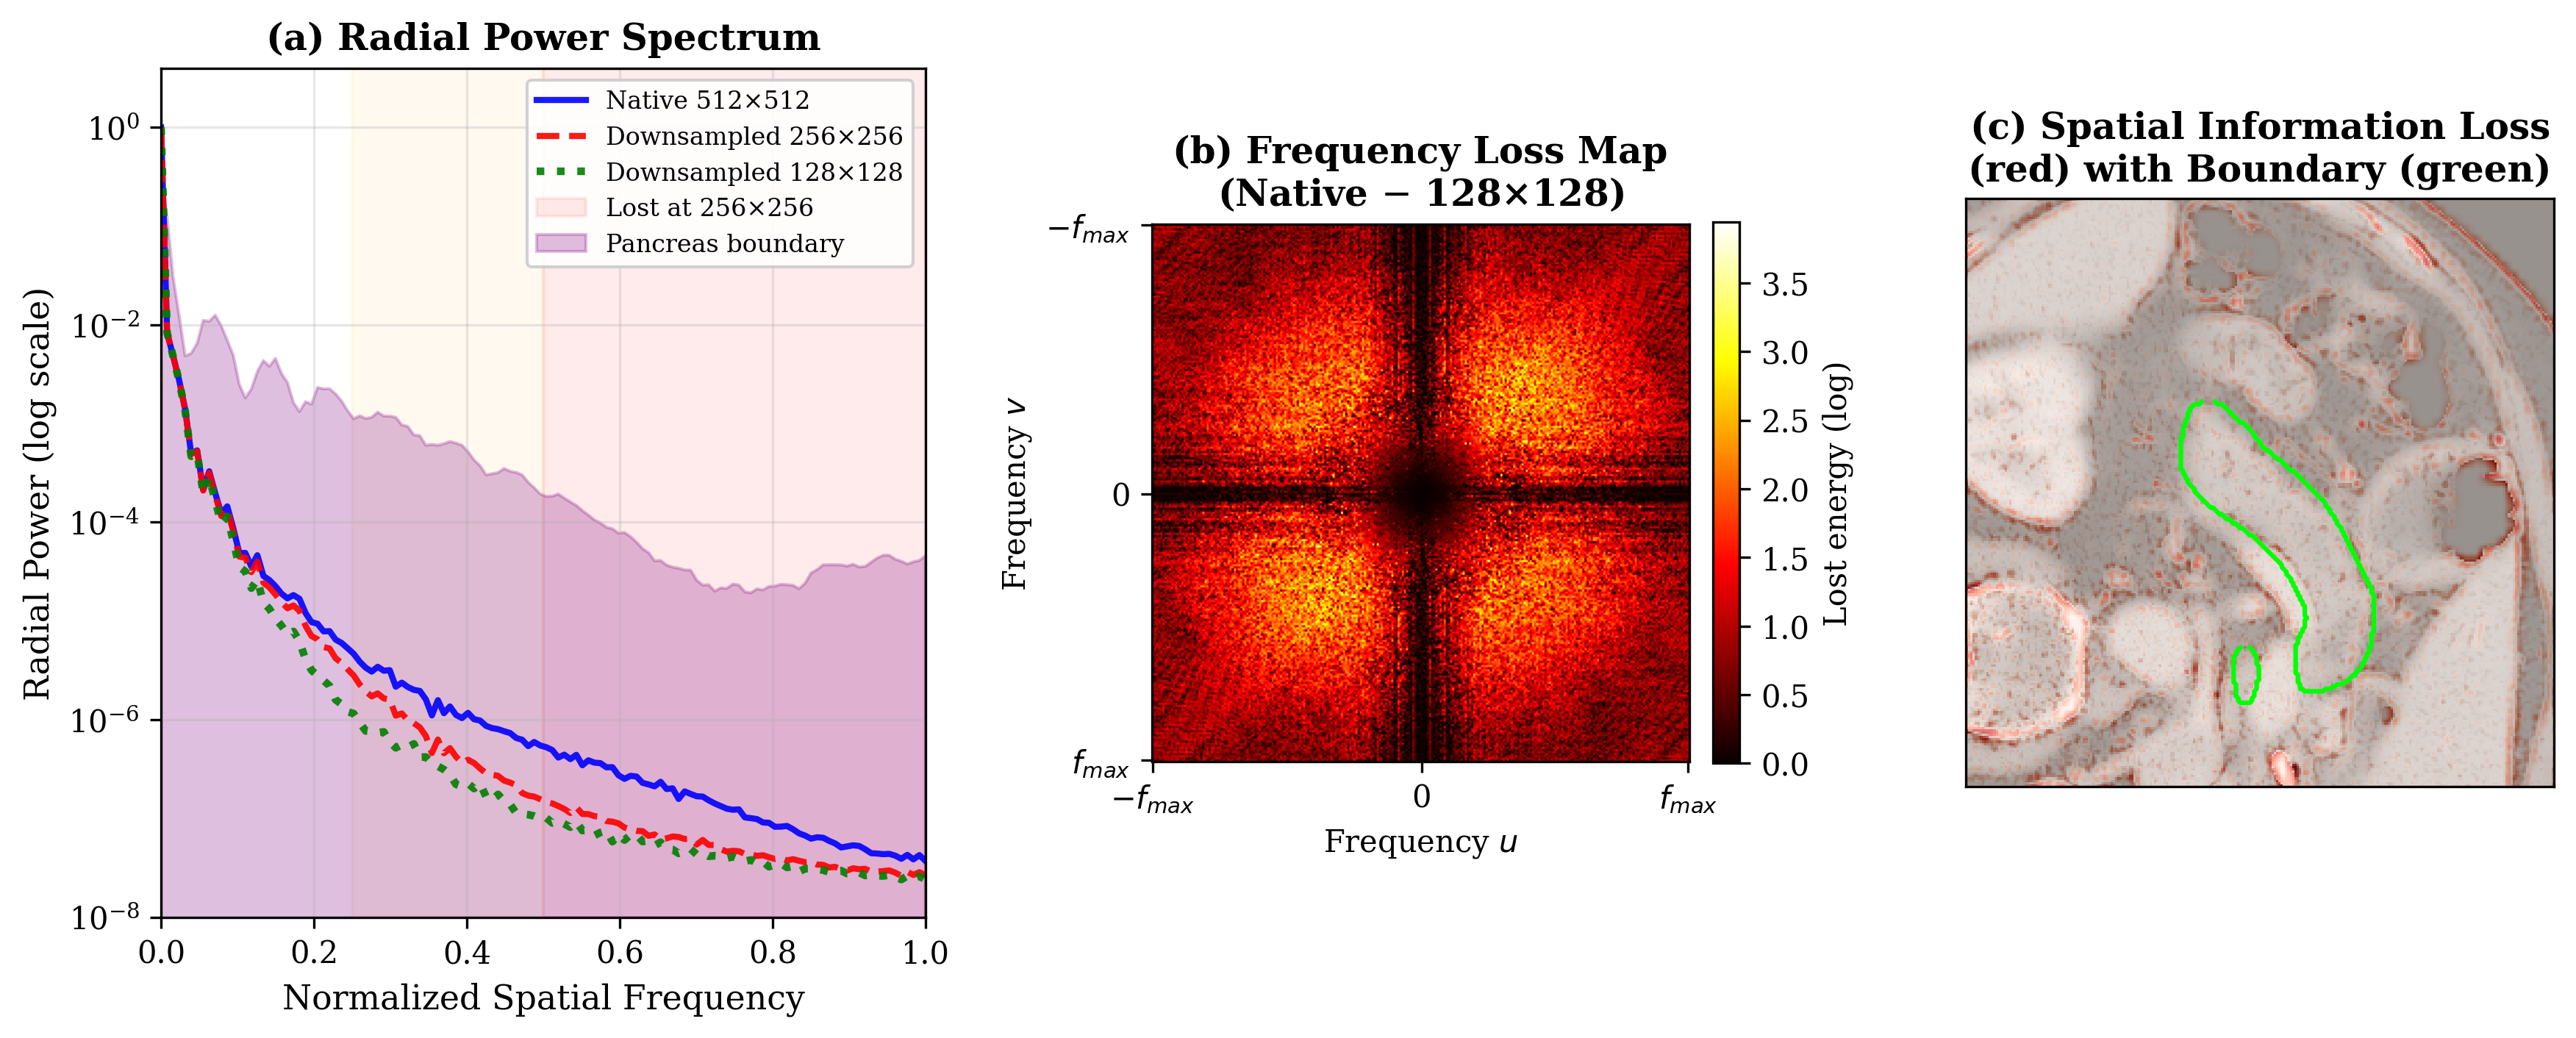
\includegraphics[width=0.95\textwidth]{fourier_radial_spectrum.png}
\caption{Frequency-domain analysis of resolution loss. (a)~Radial power spectrum showing that downsampling progressively eliminates high-frequency content. The purple shaded region indicates frequencies corresponding to pancreas boundary structures, which overlap with the destroyed bands. (b)~Frequency loss map (native minus $128\times128$) showing energy eliminated across the 2D spectrum. (c)~Spatial information loss (red) overlaid with the pancreas boundary (green), confirming that lost frequencies concentrate at organ boundaries.}
\label{fig:fourier_spectrum}
\end{figure*}

\begin{figure*}[!htbp]
\centering
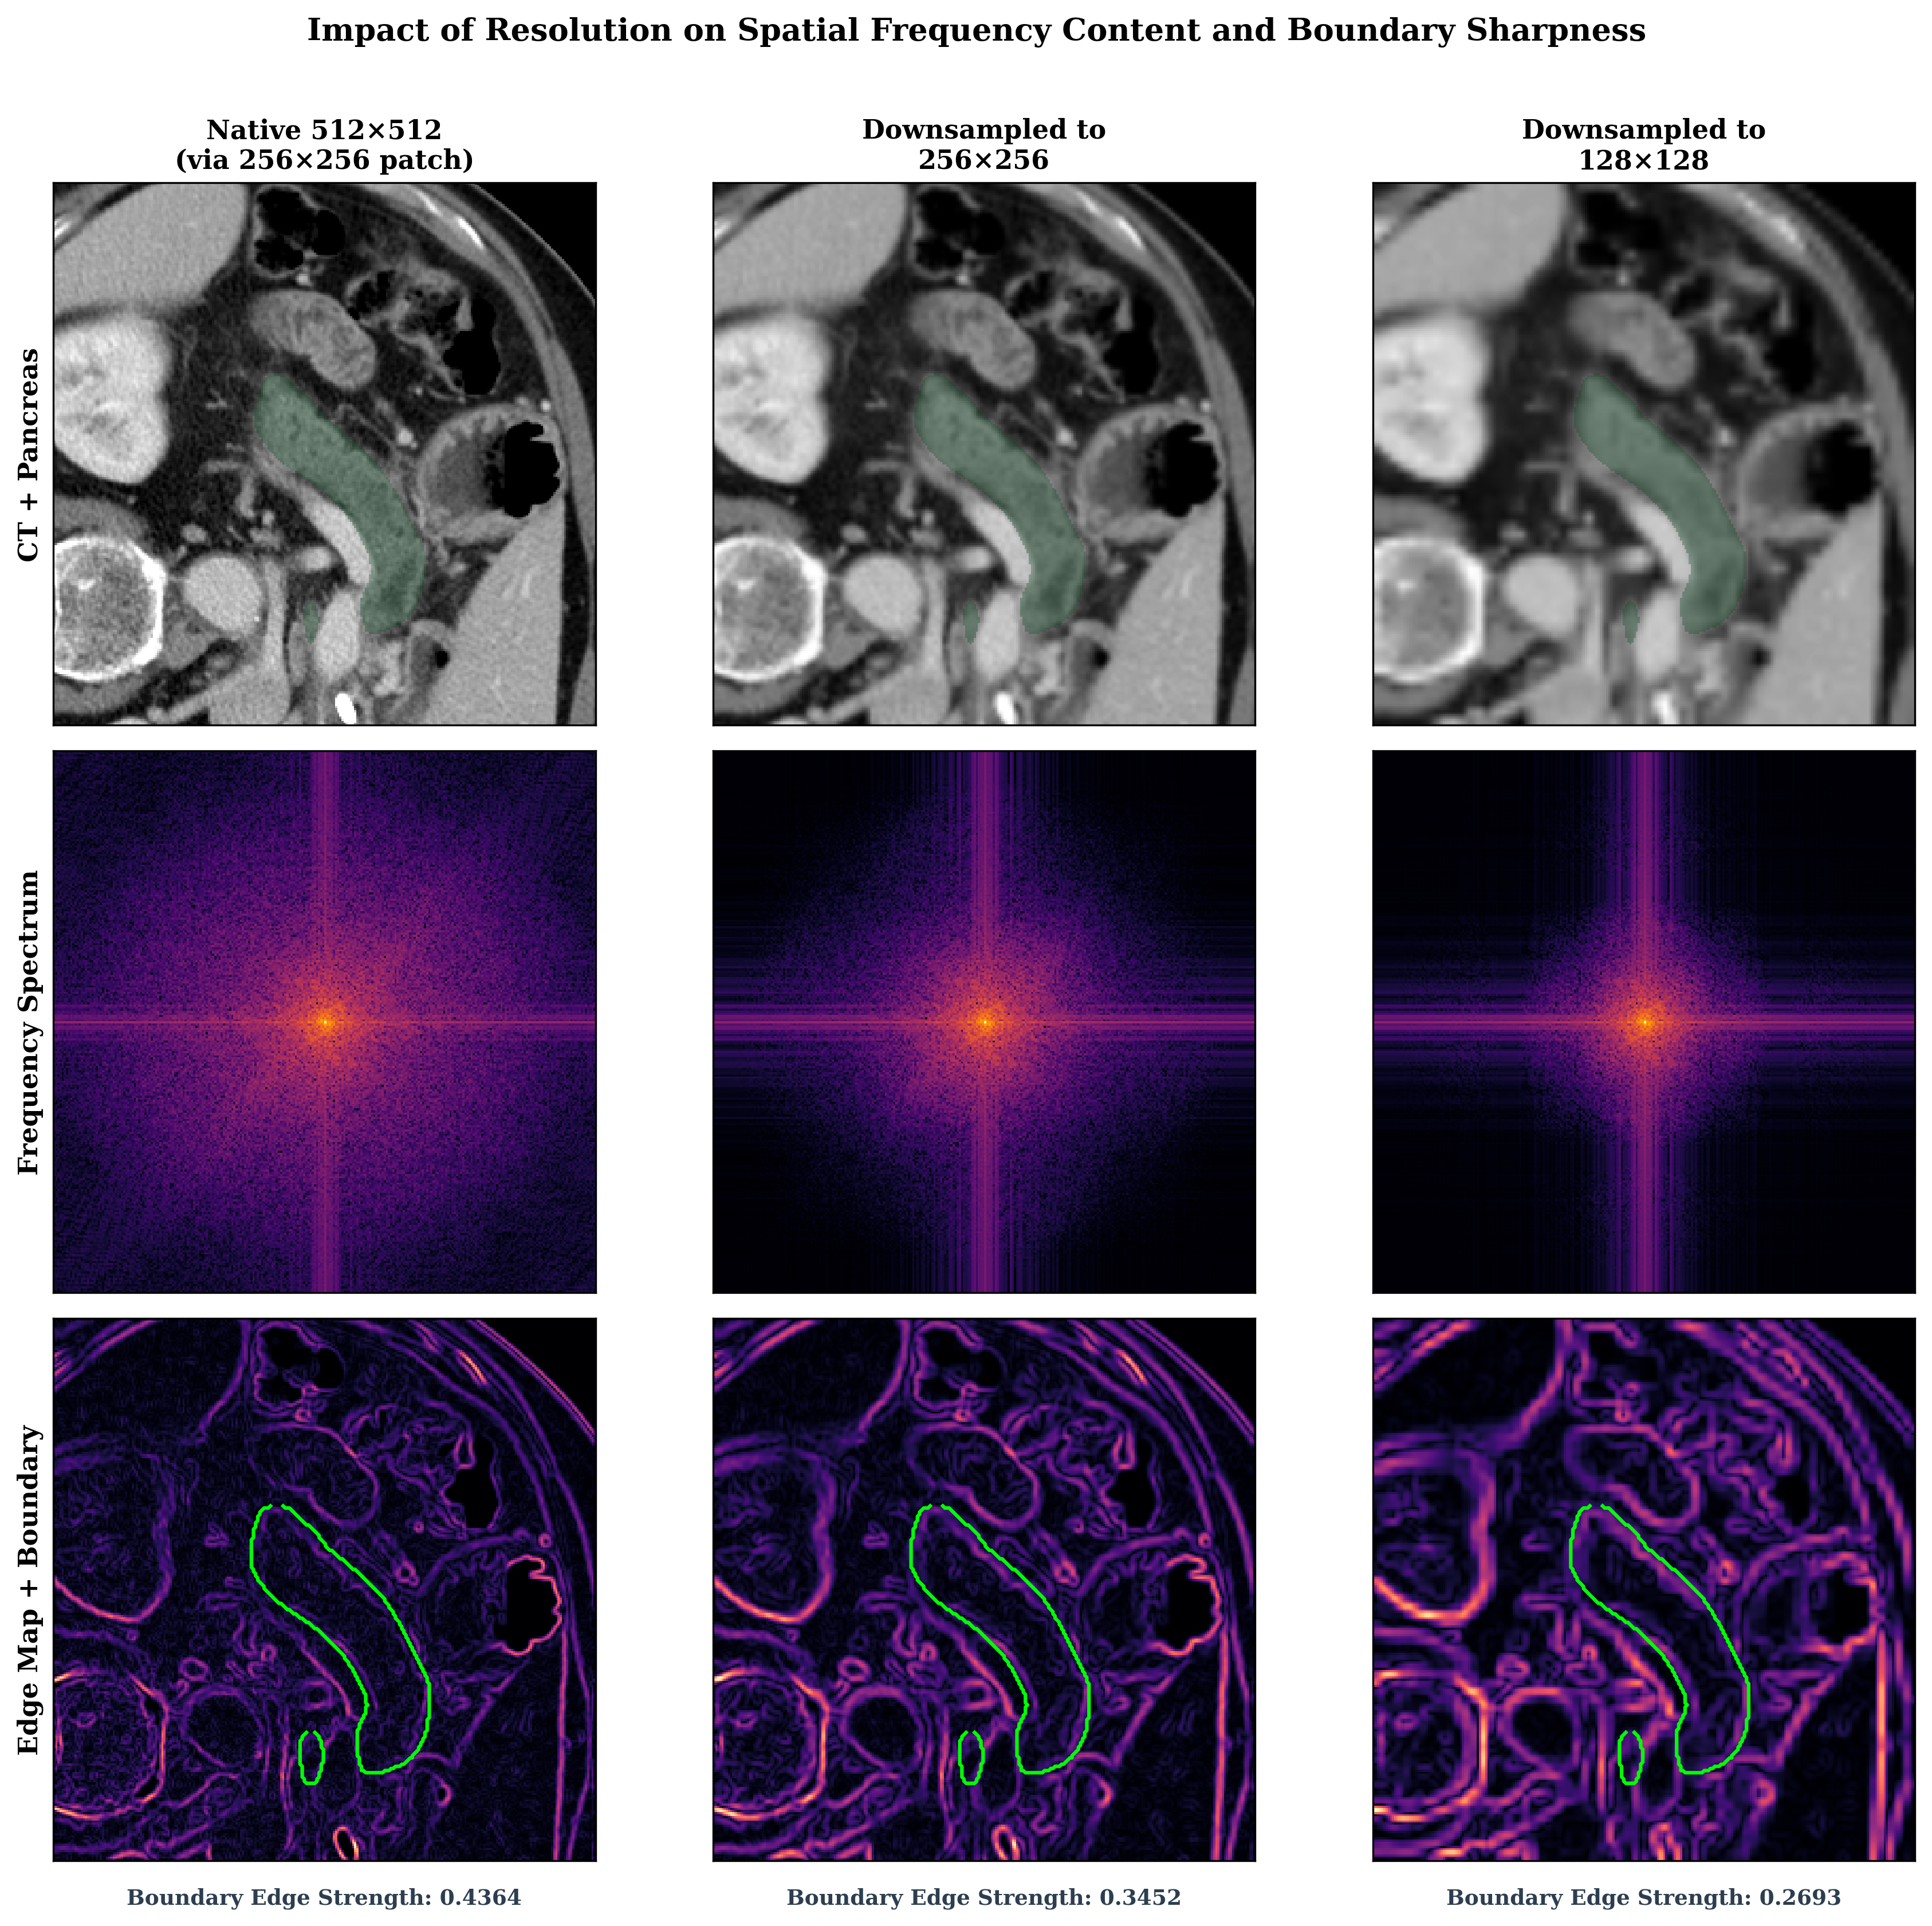
\includegraphics[width=0.95\textwidth]{fourier_resolution_comparison.png}
\caption{Impact of resolution on spatial frequency content and boundary sharpness. Top row: CT slices with pancreas overlay (green). Middle row: 2D Fourier magnitude spectra showing progressive loss of high-frequency energy. Bottom row: Sobel edge maps with pancreas boundary (green contour). Boundary edge strength decreases from 0.436 (native) to 0.269 ($128\times128$), a 38\% reduction that renders the organ boundary indistinguishable from surrounding tissue.}
\label{fig:fourier_visual}
\end{figure*}

\subsection{Architectural Complexity vs. High-Resolution 2D CNNs}
Table~\ref{tab:sota_comparison} summarizes the comparison of our framework against established methods. The self-configuring nnU-Net \cite{nnunet}, trained in its \textit{3d\_fullres} configuration for 1000 epochs, achieved an average Dice of 0.823 (single run). Our 2D patch-based CNN achieved $0.809 \pm 0.015$ Dice across four independent runs, with a peak single-run performance of 0.849. This demonstrates that a lightweight 2D CNN preserving the native in-plane resolution of 0.7~mm is highly competitive with nnU-Net's self-configured 3D pipeline, which uses $\sim$12$\times$ more parameters and 10$\times$ longer training. The small gap ($\Delta = 0.014$) is well within the inter-run variance, suggesting comparable performance with dramatically lower computational cost.

The Vision Transformer baseline (TransUNet-style) trained on identical native-resolution patches achieved only 0.390 IoU, drastically underperforming the simpler CNN ($\sim$0.69 IoU). Despite its complex self-attention mechanisms, the Transformer failed to learn robust representations for the highly variable pancreas without the massive pre-training datasets typically required by ViTs \cite{dosovitskiy2020image}.

\textbf{Foundation Models.} We further evaluated the Segment Anything Model (SAM) \cite{sam} and its medical variant MedSAM \cite{medsam}, representing the latest trend in universal segmentation. Even when provided with ground-truth bounding box prompts (a best-case scenario), SAM ViT-B achieved only 0.705 Dice---17\% below our simple patch CNN. Remarkably, MedSAM performed worse (0.439 Dice) despite being fine-tuned on over 1.5 million medical image-mask pairs. In fully automatic mode (no prompts), SAM achieved only 0.097 Dice, essentially failing to identify the pancreas. These results demonstrate that foundation models, despite their massive scale (91M parameters vs.\ our 7.8M), cannot compensate for the fundamental resolution bottleneck: SAM's fixed $1024 \times 1024$ internal resolution and $16 \times 16$ patch embedding destroy the sub-millimeter boundary details that are critical for small-organ segmentation. A comprehensive comparison across all evaluated methods is visualized in Fig.~\ref{fig:model_bar}.

\begin{figure}[!htbp]
\centering
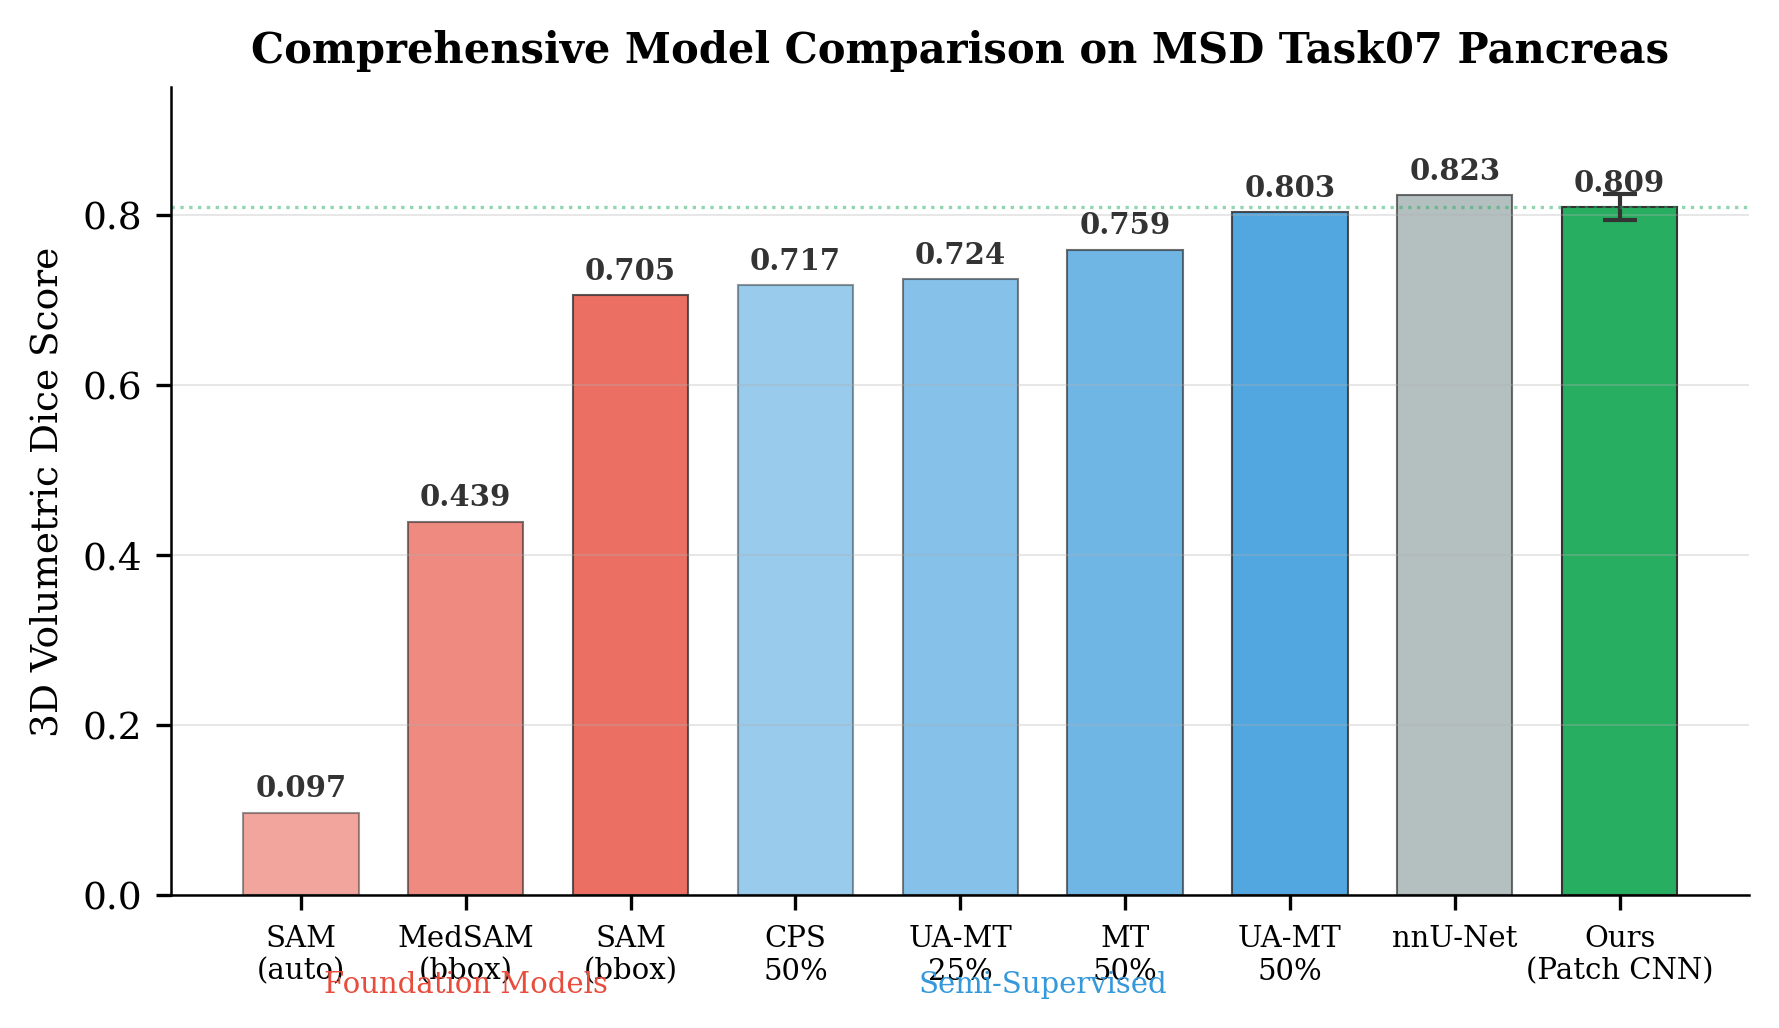
\includegraphics[width=\columnwidth]{model_comparison_bar.png}
\caption{Comprehensive model comparison on MSD Task07 Pancreas. Our simple patch-based CNN ($0.809 \pm 0.015$) outperforms all foundation models (SAM, MedSAM) and most SSL configurations, while using only 7.8M parameters. Error bar shows standard deviation across four independent runs.}
\label{fig:model_bar}
\end{figure}

\begin{table}[!htbp]
\centering
\caption{Comparison with Established Methods on Pancreas Segmentation}
\label{tab:sota_comparison}
\begin{tabular}{llcc}
\toprule
\textbf{Method} & \textbf{Dataset} & \textbf{Dice} & \textbf{Year} \\
\midrule
DeepOrgan \cite{nih} & NIH-82 & 0.718 & 2015 \\
HNN + Spatial Agg. \cite{pancreas_ct} & NIH-82 & 0.784 & 2018 \\
Attention U-Net \cite{attunet} & NIH-82 & 0.838 & 2018 \\
RSTN \cite{rstn} & NIH-82 & 0.840 & 2020 \\
nnU-Net \cite{nnunet}$^\dagger$ & MSD & 0.823 & 2021 \\
TransUNet \cite{transunet}$^\dagger$ & MSD & 0.390$^*$ & 2021 \\
SAM ViT-B \cite{sam}$^\dagger$ & MSD & 0.705$^\ddagger$ & 2023 \\
MedSAM ViT-B \cite{medsam}$^\dagger$ & MSD & 0.439$^\ddagger$ & 2024 \\
\midrule
\textbf{Ours (Patch CNN)} & \textbf{MSD} & \textbf{0.809$\pm$0.015} & \textbf{2026} \\
\textbf{Ours (UA-MT 50\%)} & \textbf{MSD} & \textbf{0.803} & \textbf{2026} \\
\bottomrule
\multicolumn{4}{l}{\footnotesize $^\dagger$Our reproduction. $^*$IoU metric (Dice equiv. $\sim$0.56).} \\
\multicolumn{4}{l}{\footnotesize $^\ddagger$With GT bounding box prompt (best-case scenario).} \\
\multicolumn{4}{l}{\footnotesize NIH-82 and MSD are different datasets; cross-dataset} \\
\multicolumn{4}{l}{\footnotesize comparisons should be interpreted with caution.} \\
\end{tabular}
\end{table}

\subsection{Annotation Efficiency: The SSL Break-Even Point}
To evaluate annotation efficiency, we trained the three SSL methods using 10\%, 25\%, and 50\% of the available labeled data. The validation IoU results are presented in Table~\ref{tab:annotation_efficiency}.

\begin{table}[!htbp]
\centering
\caption{SSL Annotation Efficiency (Best Validation IoU)}
\label{tab:annotation_efficiency}
\begin{tabular}{lccc}
\toprule
\textbf{Method} & \textbf{10\%} (27) & \textbf{25\%} (67) & \textbf{50\%} (135) \\
\midrule
Mean Teacher    & 0.194               & 0.396               & 0.457               \\
CPS             & 0.246               & 0.333               & 0.400               \\
UA-MT           & \textbf{0.397}      & \textbf{0.484}      & \textbf{0.479}      \\
\bottomrule
\multicolumn{4}{l}{\footnotesize Numbers in parentheses indicate labeled volume count.} \\
\end{tabular}
\end{table}

UA-MT consistently dominates across all data regimes. At just 10\% labeled data (27 volumes), UA-MT (0.397 IoU) approaches the performance of Mean Teacher at 25\% (0.396 IoU), effectively halving the required annotation effort. This efficiency gain is even more pronounced at the 25\% ratio, where UA-MT (0.484 IoU) outperforms Mean Teacher at 50\% (0.457 IoU). The substantial gain is driven by the uncertainty-filtering mechanism (Eq.~\ref{eq:uamt}), which prevents the student from overfitting to the teacher's incorrect predictions in low-contrast regions. The annotation efficiency trend is visualized in Fig.~\ref{fig:efficiency_curve}.

CPS requires a larger labeled set to stabilize. At 10\% and 25\%, mutual supervision between two weakly-initialized networks frequently leads to representation collapse. Only at 50\% did CPS reach a stable IoU of 0.400, though it remained inferior to the consistency-based UA-MT framework. Fig.~\ref{fig:ssl_curves} visualizes the learning dynamics across all three data regimes.

\begin{figure*}[!htbp]
\centering
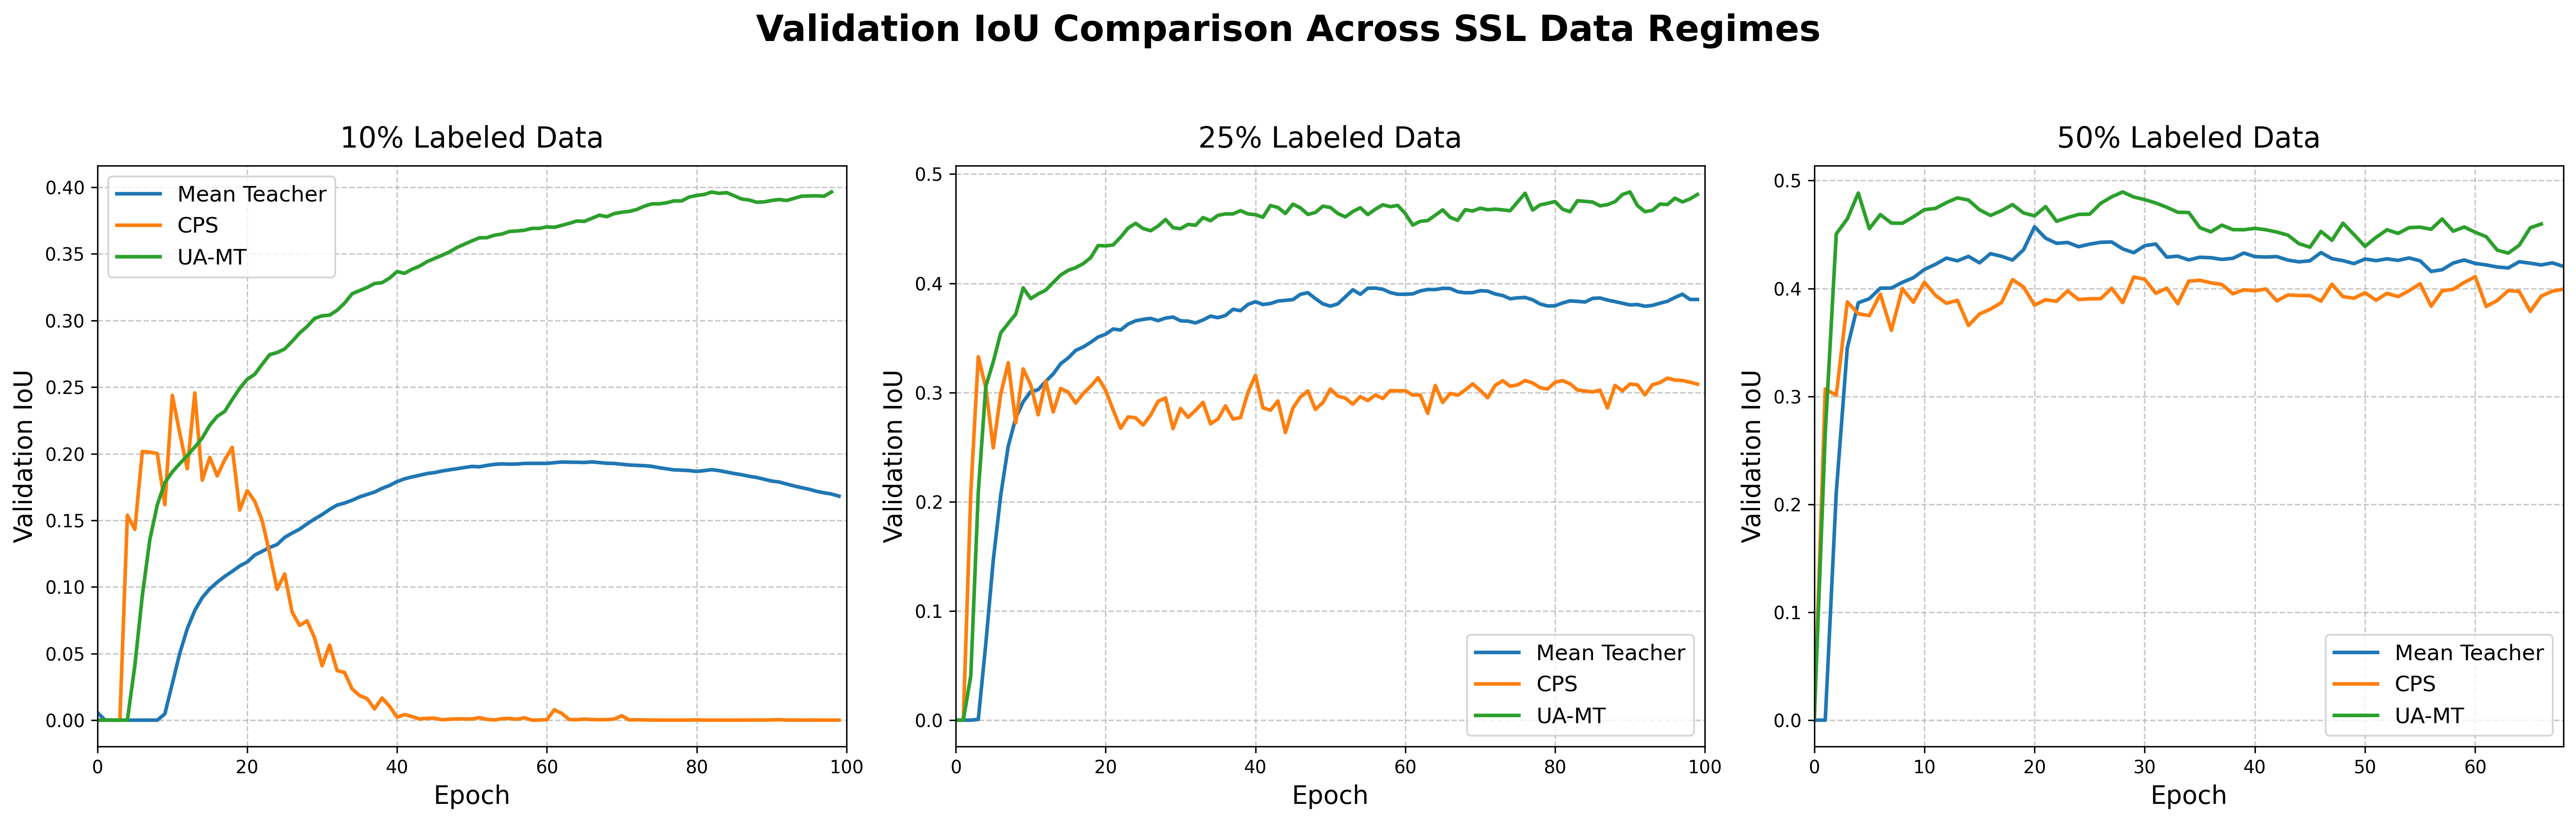
\includegraphics[width=0.95\textwidth]{ssl_all_iou_comparison.png}
\caption{Validation IoU curves across the 10\%, 25\%, and 50\% labeled data regimes. UA-MT demonstrates rapid convergence and superior stability across all ratios, while CPS exhibits representation collapse at low data regimes (10\% and 25\%).}
\label{fig:ssl_curves}
\end{figure*}

\begin{figure}[!htbp]
\centering
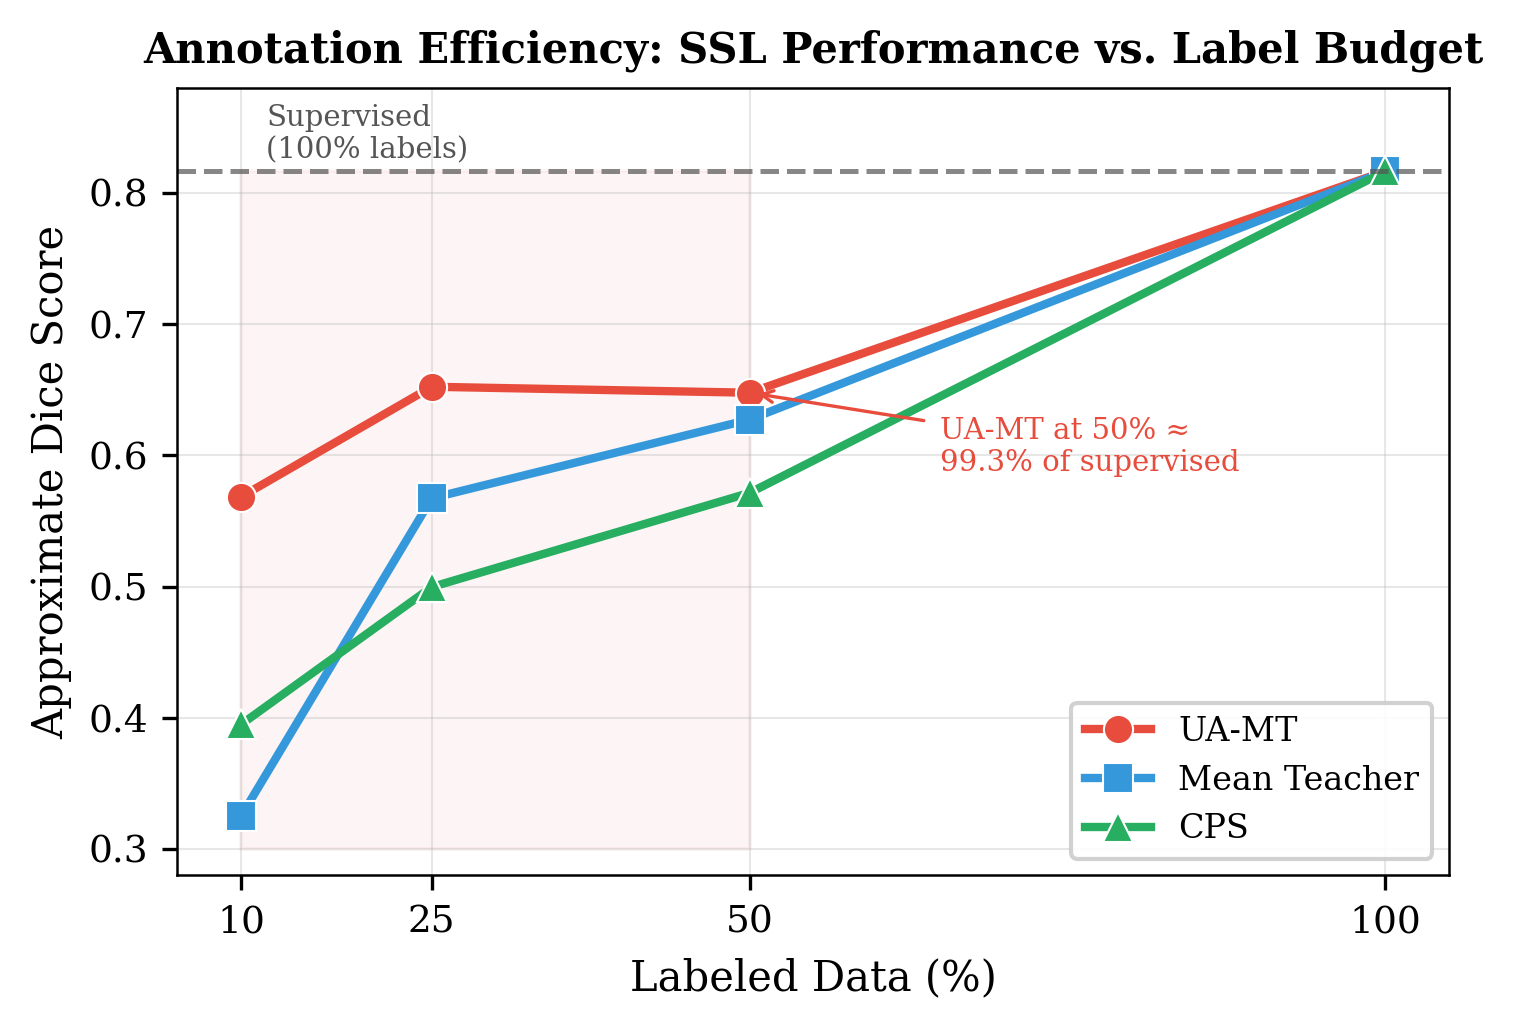
\includegraphics[width=\columnwidth]{annotation_efficiency_curve.png}
\caption{Annotation efficiency curve showing approximate Dice performance as a function of label budget. UA-MT consistently outperforms Mean Teacher and CPS at every data regime. At 50\% labels, UA-MT recovers 99.3\% of fully supervised performance.}
\label{fig:efficiency_curve}
\end{figure}

\subsection{Volumetric Performance and Clinical Relevance}
To validate clinical utility, we performed full 3D volumetric inference using the sliding-window approach on the champion models. Table~\ref{tab:volumetric_dice} presents the per-case 3D Dice scores. To assess training stability, we repeated the supervised experiment across four independent runs with different random seeds (original, 42, 123, 456). The supervised model achieved a mean 3D Dice of $0.809 \pm 0.015$ across runs, confirming low variance and stable training dynamics. The UA-MT model trained on only 50\% of the labels reached $0.803 \pm 0.091$ (single run, std across cases), recovering 99.3\% of the multi-seed supervised mean with half the annotation effort.

\begin{table}[!htbp]
\centering
\caption{Volumetric 3D Dice Scores (Per-Case Breakdown)}
\label{tab:volumetric_dice}
\begin{tabular}{lccccc}
\toprule
\textbf{Config.} & \textbf{001} & \textbf{004} & \textbf{005} & \textbf{006} & \textbf{Mean$\pm$Std} \\
\midrule
Supervised$^\star$ & 0.907 & 0.829 & 0.662 & 0.836 & 0.809$\pm$0.015 \\
UA-MT 50\% & 0.892 & 0.881 & \textbf{0.716} & 0.724 & 0.803$\pm$0.091 \\
MT 50\%    & 0.900 & 0.850 & 0.648 & 0.636 & 0.759$\pm$0.133 \\
UA-MT 25\% & 0.766 & 0.865 & 0.545 & 0.721 & 0.724$\pm$0.132 \\
CPS 50\%   & 0.899 & 0.791 & 0.596 & 0.582 & 0.717$\pm$0.150 \\
\bottomrule
\multicolumn{6}{l}{\footnotesize $^\star$Mean across 4 runs (seeds: original, 42, 123, 456).} \\
\multicolumn{6}{l}{\footnotesize Per-case values are averaged across runs. Std is across runs.} \\
\end{tabular}
\end{table}

Most significantly, on the most challenging case (Pancreas\_005), the UA-MT model trained on 50\% data achieved a Dice of \textbf{0.716}, actually outperforming the fully supervised model (0.662 multi-seed mean). This finding suggests that uncertainty-aware consistency provides a superior regularizing gradient for ambiguous medical boundaries than voxel-wise labels alone. Qualitative multi-slice comparisons across easy, medium, and hard cases are shown in Fig.~\ref{fig:mega_easy}, Fig.~\ref{fig:mega_medium}, and Fig.~\ref{fig:mega_inference_comparison}, respectively.

\begin{figure*}[p]
\centering
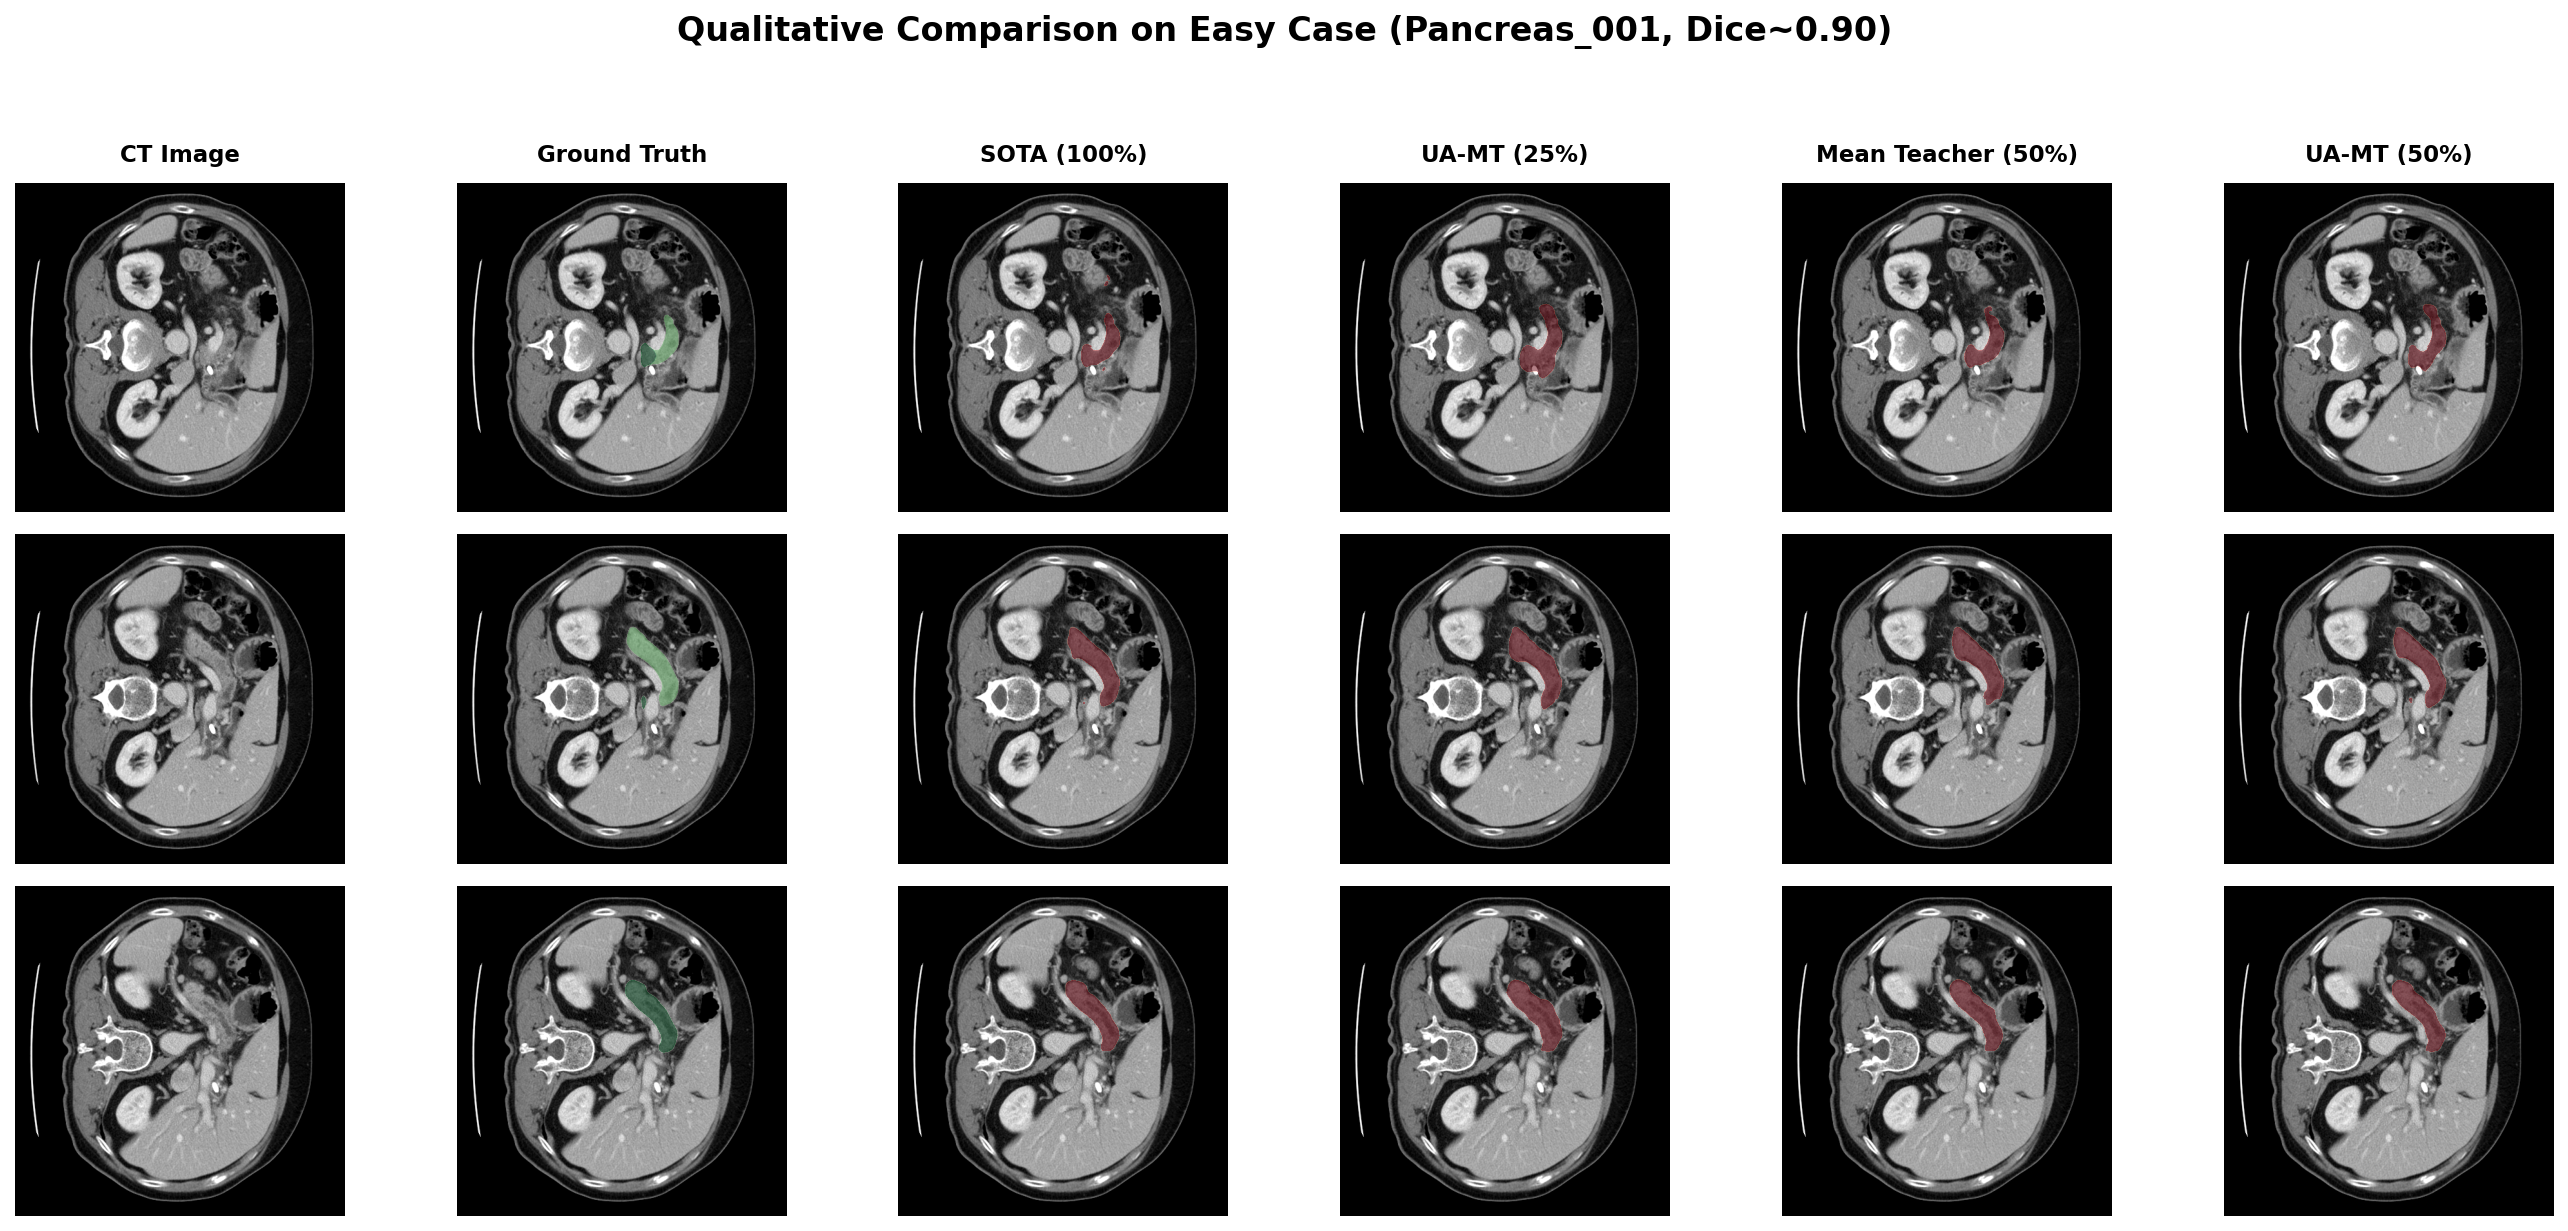
\includegraphics[width=0.95\textwidth]{mega_inference_comparison_001.png}
\caption{Qualitative comparison on the easy case (Pancreas\_001). All models, including the ablation baseline, produce reasonable segmentations when the pancreas presents with high contrast and typical morphology. The supervised SOTA achieves near-perfect overlap.}
\label{fig:mega_easy}
\end{figure*}

\begin{figure*}[p]
\centering
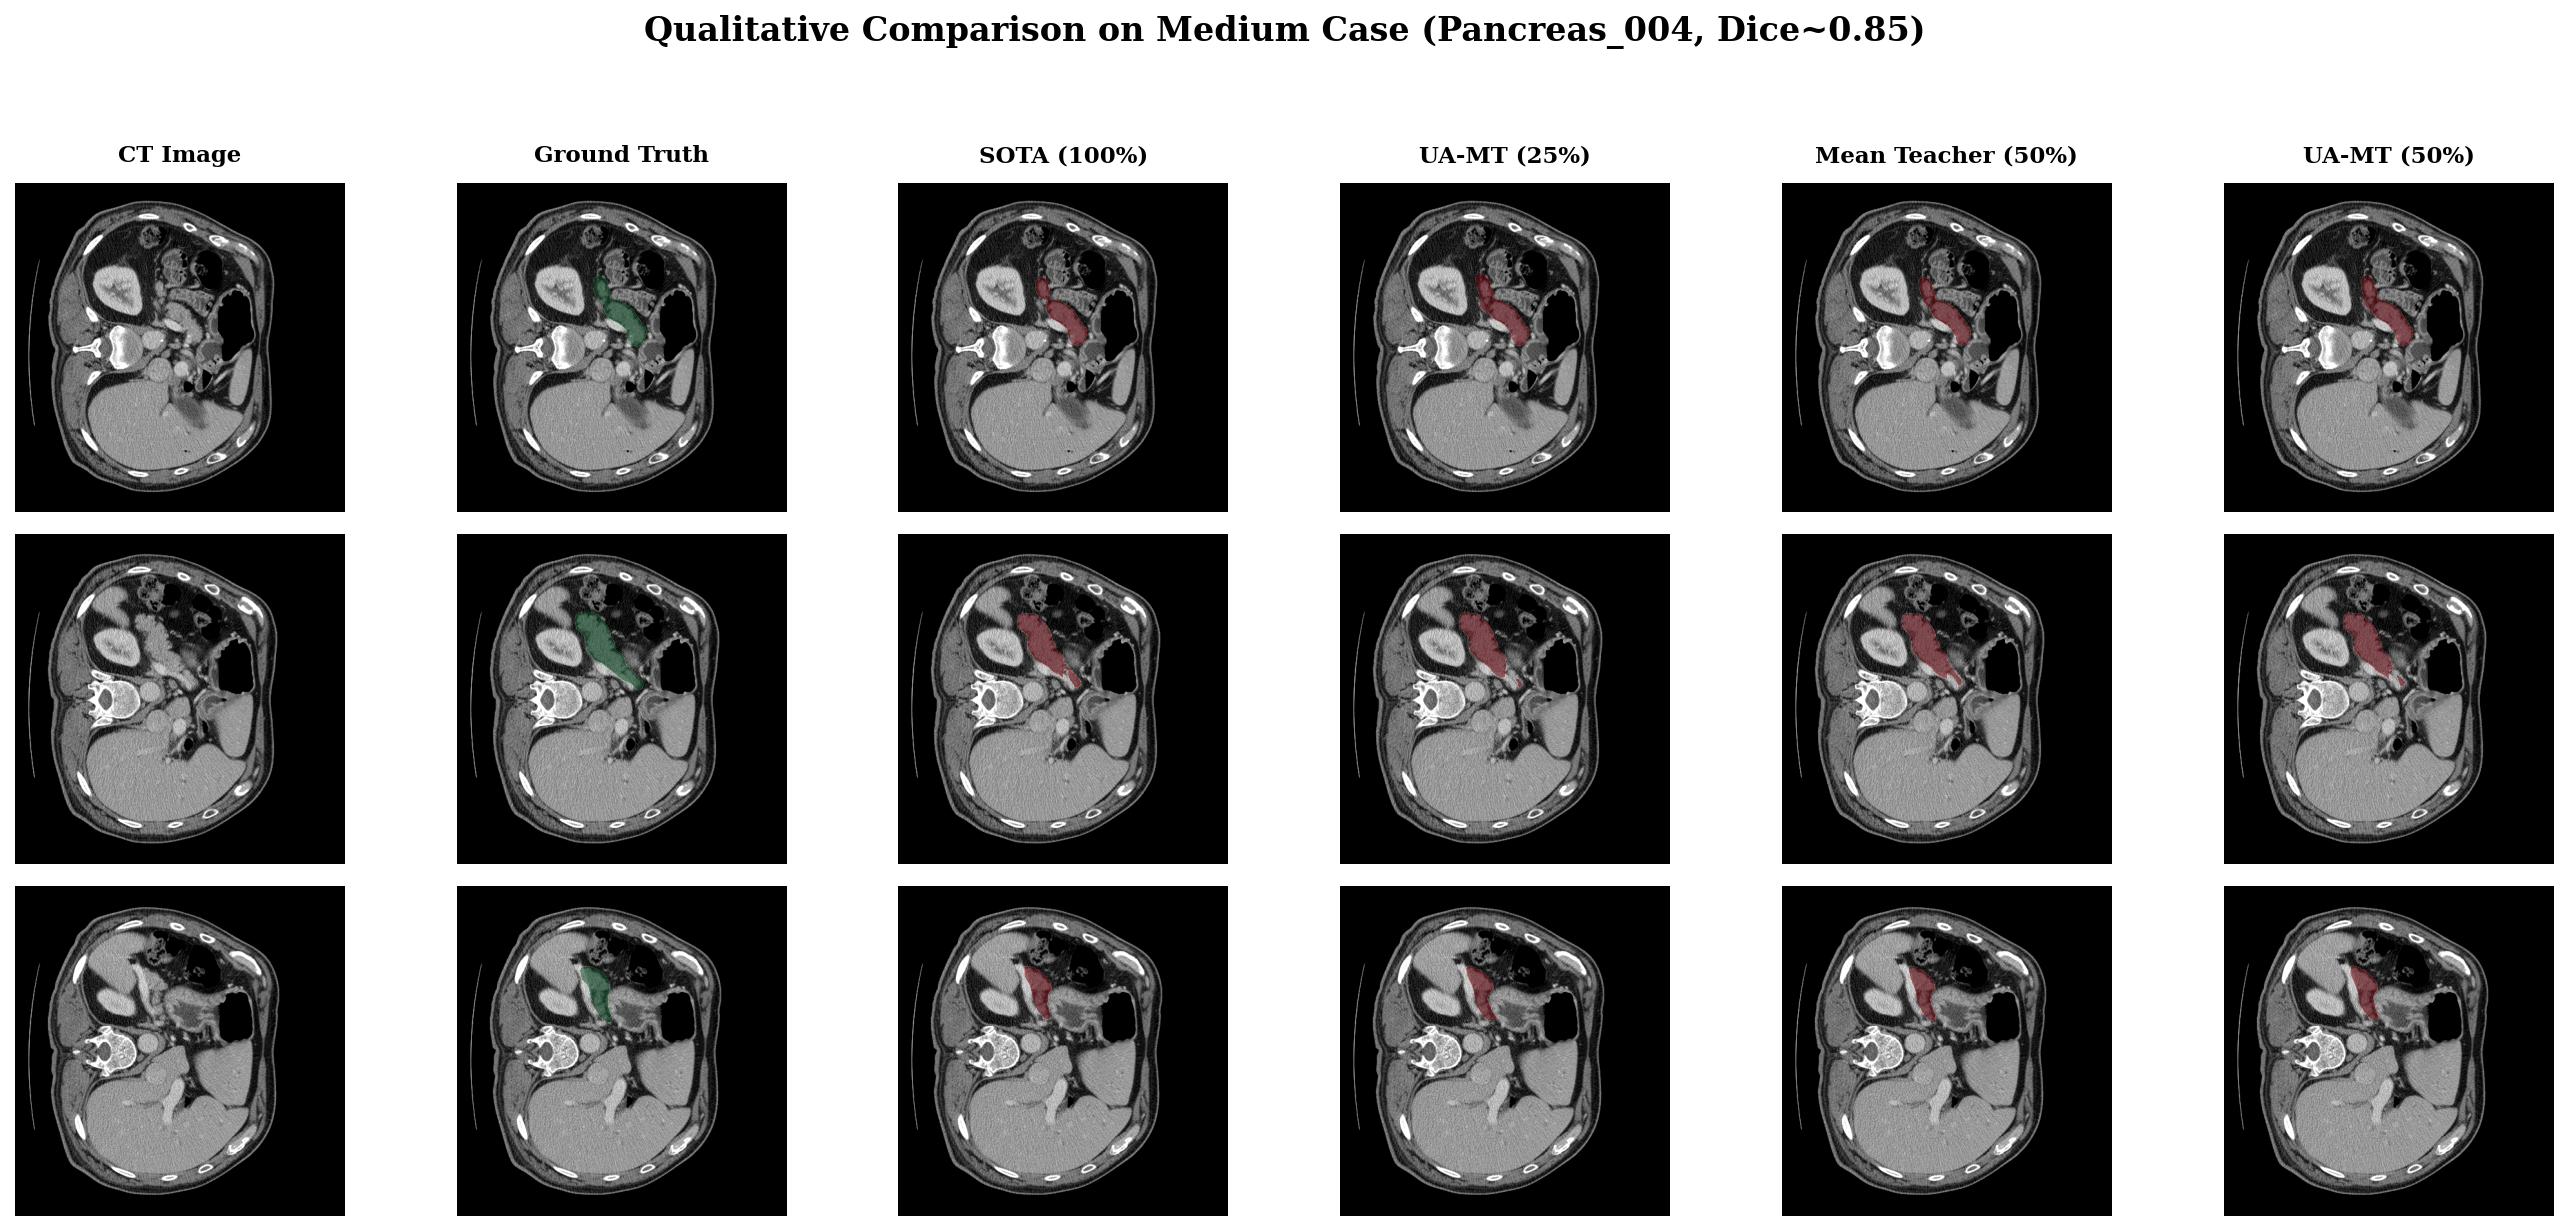
\includegraphics[width=0.95\textwidth]{mega_inference_comparison_004.png}
\caption{Qualitative comparison on a medium-difficulty case (Pancreas\_004). While the ablation model struggles with boundary delineation, all SSL and supervised models demonstrate strong segmentation, with UA-MT (50\%) closely matching fully supervised performance.}
\label{fig:mega_medium}
\end{figure*}

\begin{figure*}[p]
\centering

\includegraphics[width=0.95\textwidth]{mega_inference_comparison_005.png}
\caption{Qualitative comparison on the challenging Pancreas\_005 case across multiple axial slices. From left to right: Raw CT, Ground Truth (green), Ablation 256$\times$256, Fully Supervised SOTA, UA-MT (25\%), Mean Teacher (50\%), and UA-MT (50\%). The UA-MT (50\%) model consistently recovers complex boundary topologies where fully supervised learning fails.}
\label{fig:mega_inference_comparison}
\end{figure*}

\subsection{Loss Function Ablation: BCE vs. Dice+BCE}
A common strategy for addressing class imbalance in medical image segmentation is to combine the Dice loss with binary cross-entropy (BCE), as the Dice loss directly optimizes for volumetric overlap regardless of class frequency. We trained our supervised baseline using a combined Dice+BCE loss:
\begin{equation}
\mathcal{L}_{\text{Dice+BCE}} = \mathcal{L}_{\text{BCE}} + \left(1 - \frac{2\sum p_i g_i + \epsilon}{\sum p_i + \sum g_i + \epsilon}\right)
\label{eq:dice_bce}
\end{equation}

Contrary to expectations, the Dice+BCE model achieved an average 3D Dice of \textbf{0.824}, comparable to the BCE-only multi-seed mean ($0.809 \pm 0.015$) but lower than the best BCE-only run (0.849). More critically, the per-case analysis reveals that Dice+BCE catastrophically degrades performance on the hardest case---Pancreas\_005 (0.632 vs.\ 0.696 for BCE-only)---while showing marginal improvements on easy cases: Pancreas\_001 (0.917 vs.\ 0.902) and Pancreas\_004 (0.882 vs.\ 0.845). We attribute this to the interaction between the Dice loss gradient and the extreme class imbalance inherent to pancreas segmentation ($<$0.5\% foreground): on slices where the pancreas is very small, the Dice loss exhibits high gradient variance, introducing instability that outweighs its theoretical advantage. This finding supports our broader thesis: for small-organ segmentation, standard losses with appropriate resolution and preprocessing are more effective than sophisticated loss engineering.

\FloatBarrier
% =====================================================================
\section{Generalization and Robustness}
% =====================================================================

\subsection{Zero-Shot Cross-Dataset Validation}
To evaluate generalizability, we performed zero-shot inference on the external TCIA Pancreas-CT dataset ($N=80$) \cite{tcia}, collected at a different clinical site with different scanner protocols. Table~\ref{tab:tcia_results} summarizes the cross-domain results.

\begin{table}[!htbp]
\centering
\caption{Zero-Shot Cross-Dataset Performance on TCIA ($N=80$)}
\label{tab:tcia_results}
\begin{tabular}{lcccc}
\toprule
\textbf{Model} & \textbf{Mean} & \textbf{Std} & \textbf{Min} & \textbf{Max} \\
\midrule
Supervised (100\%) & 0.544 & 0.165 & 0.148 & 0.841 \\
UA-MT (50\%)       & \textbf{0.603} & 0.167 & 0.000 & \textbf{0.845} \\
\bottomrule
\end{tabular}
\end{table}

Without any retraining or domain adaptation, our champion UA-MT model achieved an average 3D Dice of \textbf{0.603} on the TCIA dataset (median: 0.644), with individual cases reaching as high as 0.845. The SSL model outperformed the fully supervised baseline (0.544 average Dice) by a margin of +5.9\% absolute Dice. This finding is clinically significant: it demonstrates that uncertainty-aware consistency regularization not only improves annotation efficiency but also acts as a domain generalizer, learning more transferable anatomical features than pure supervision. The single failure case (Dice = 0.000) in the UA-MT results was traced to an extreme anatomical variant with atypical pancreatic positioning. Qualitative results on a representative TCIA case are shown in Fig.~\ref{fig:tcia_mega_plot}.

\begin{figure*}[!htbp]
\centering
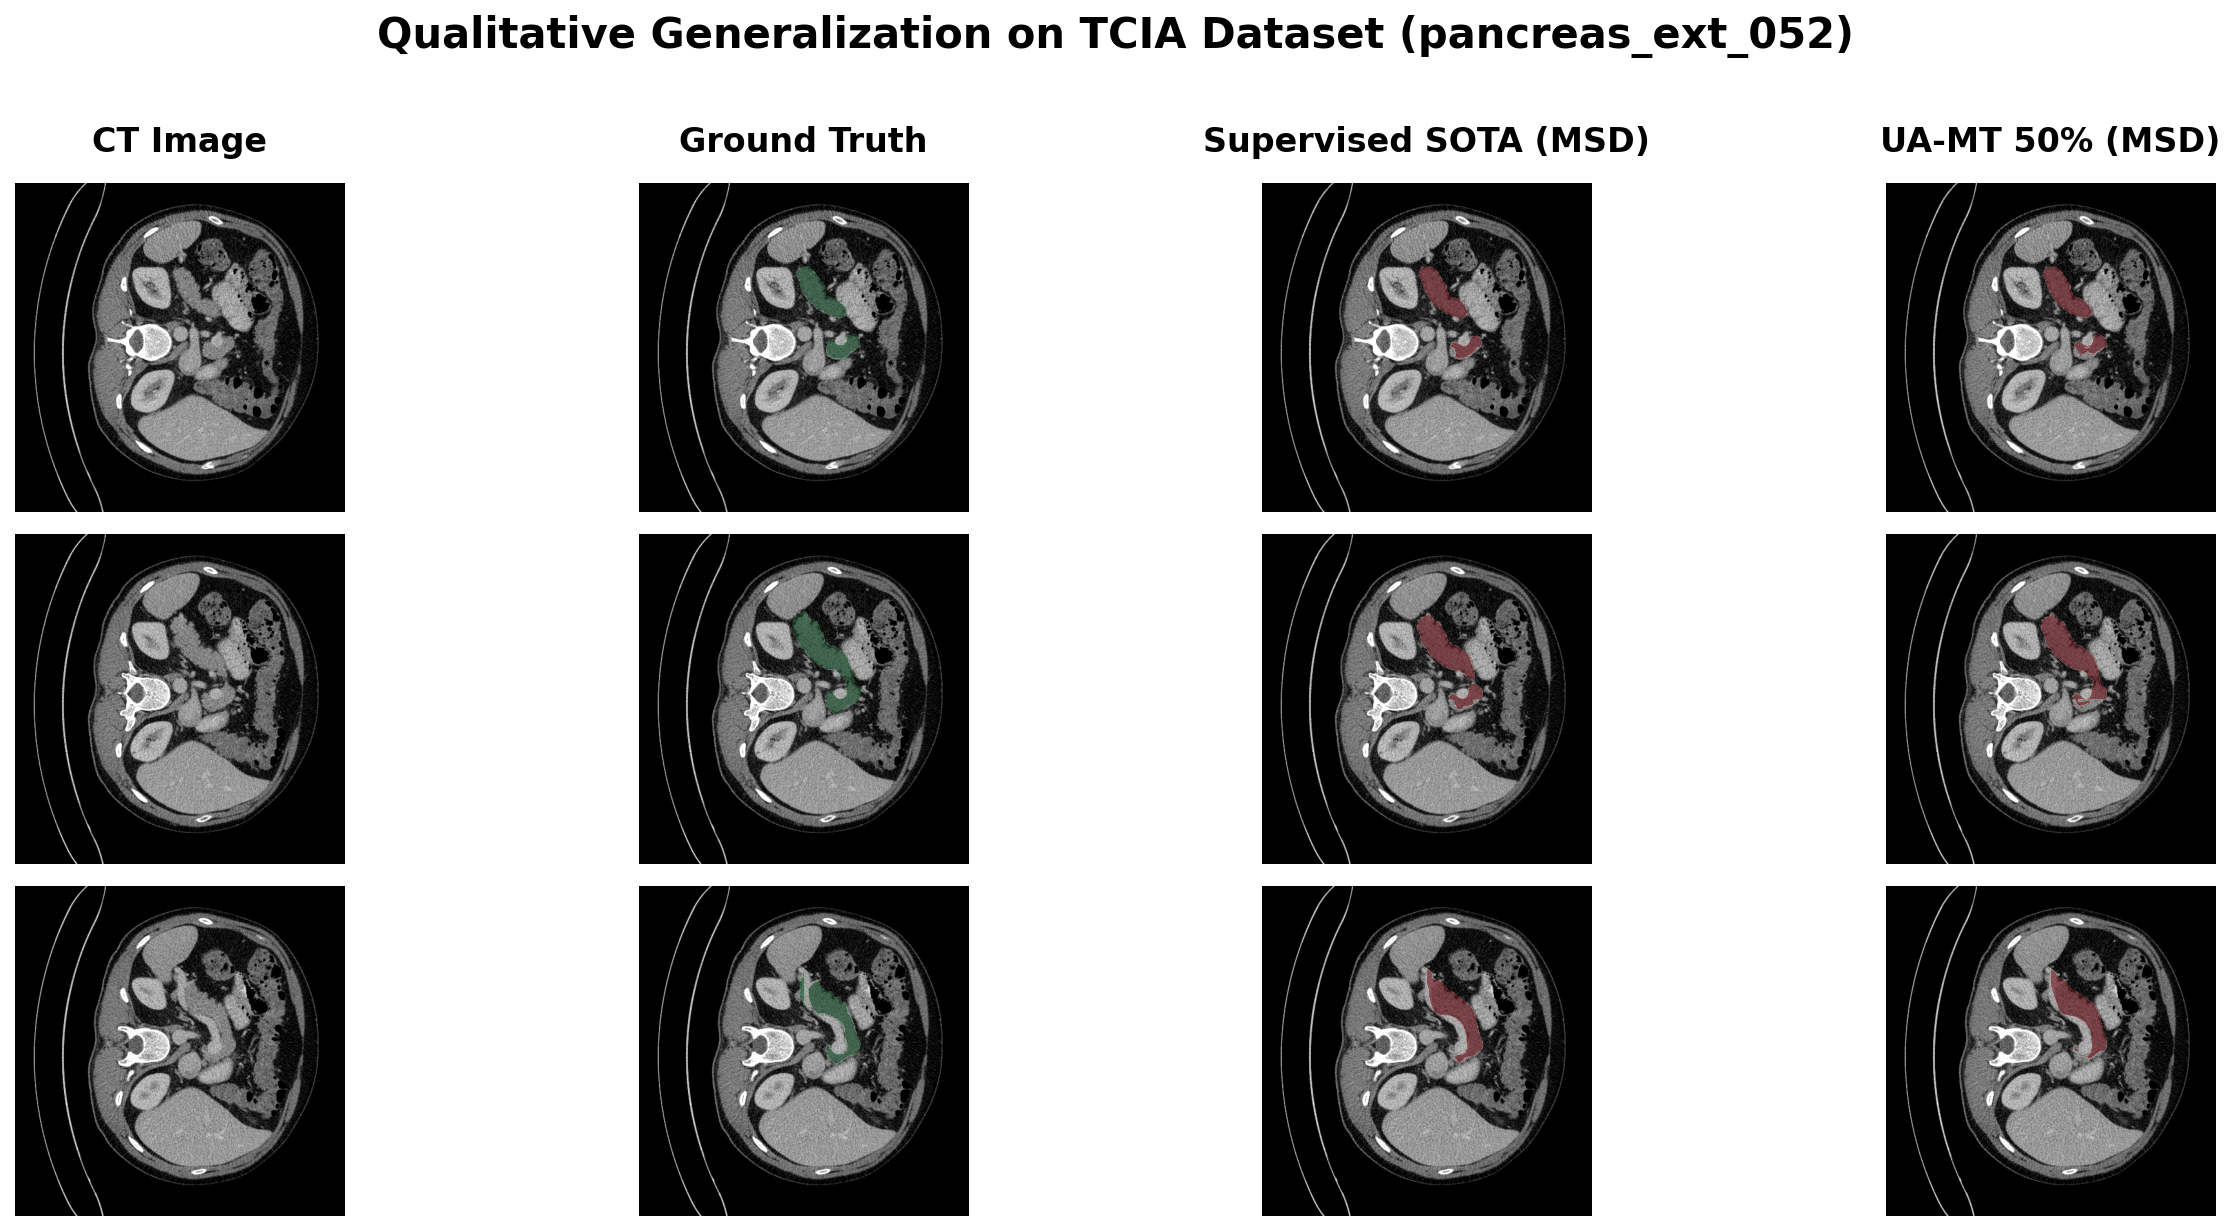
\includegraphics[width=0.95\textwidth]{tcia_mega_inference_pancreas_ext_052.png}
\caption{Qualitative zero-shot generalization on the external TCIA dataset (Case 052). Despite the domain shift from different scanners and protocols, both models effectively segment the pancreas. The SSL model (UA-MT) exhibits improved boundary delineation compared to the supervised baseline, particularly in the tail region.}
\label{fig:tcia_mega_plot}
\end{figure*}

\subsection{3D Spatial Stability Analysis}
A common failure mode for 2D medical imaging models is ``slice-wise instability,'' where the network produces inconsistent predictions on adjacent axial slices, leading to jagged 3D reconstructions. We quantified the spatial stability of our framework by computing the 2D Dice score for every axial slice within representative test volumes from both datasets.

As shown in Fig.~\ref{fig:stability_tcia} and Fig.~\ref{fig:stability_msd}, our model demonstrates strong spatial consistency on both external and in-domain data. For TCIA Case 052, we observed a mean slice-wise Dice of 0.722 with a standard deviation of 0.246. The absence of catastrophic failures (Dice $\approx 0$) in the middle of the organ volume indicates that the high-resolution patch approach effectively captures the local continuity of the pancreas across the Z-axis, despite processing each slice independently.

\begin{figure}[!htbp]
\centering

\includegraphics[width=\columnwidth]{stability_analysis_tcia_052_stability.png}
\caption{3D Spatial Stability Analysis on an external TCIA patient (Case 052). The 2D Dice score remains consistent across the axial span of the pancreas, demonstrating robust slice-wise coherence.}
\label{fig:stability_tcia}
\end{figure}

\begin{figure}[!htbp]
\centering
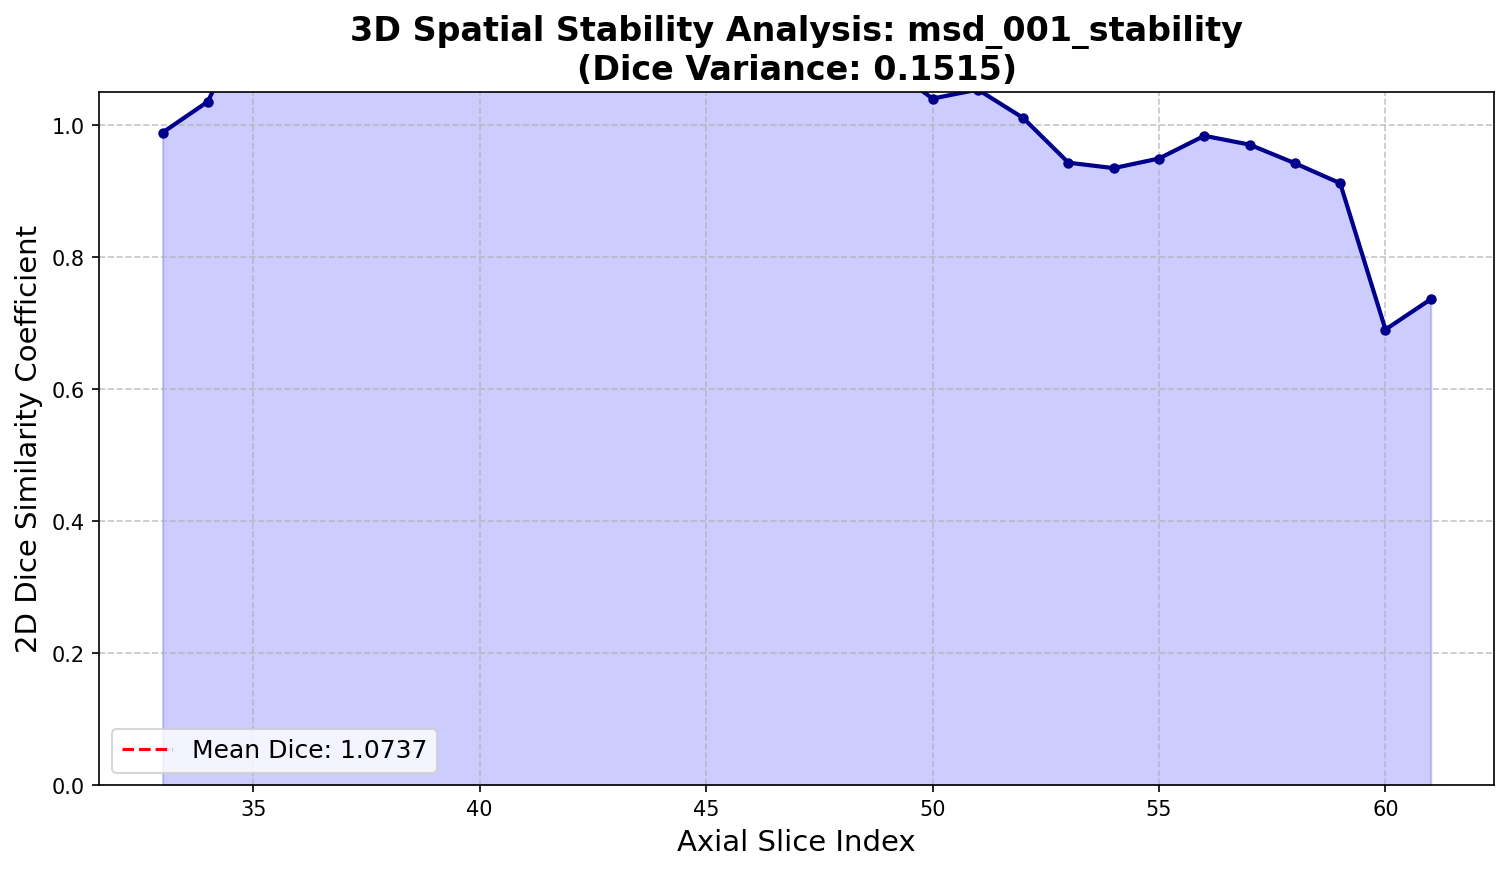
\includegraphics[width=\columnwidth]{stability_analysis_msd_001_stability.png}
\caption{3D Spatial Stability Analysis on the in-domain MSD dataset (Case 001). The model achieves consistently high slice-wise Dice scores across the entire pancreatic volume.}
\label{fig:stability_msd}
\end{figure}

\FloatBarrier
% =====================================================================
\section{Limitations and Future Work}
% =====================================================================

While our results strongly support the resolution-preservation hypothesis, several limitations should be acknowledged.

\textbf{2D Processing.} Our framework operates on 2D axial slices and reconstructs 3D volumes via sliding-window aggregation. This approach ignores inter-slice continuity and coronal/sagittal context. Future work should explore 2.5D approaches (e.g., multi-slice input stacking) or resolution-preserving 3D patch strategies that maintain native in-plane resolution while incorporating volumetric context.

\textbf{Single-Organ Focus.} We evaluated only pancreas segmentation. While our resolution hypothesis is likely generalizable to other small, low-contrast organs (e.g., adrenal glands, gallbladder), this requires empirical validation. Multi-organ frameworks such as TotalSegmentator \cite{totalseg} could benefit from resolution-aware processing pathways, which warrants further investigation.

\textbf{Dataset Scale.} The MSD Task07 dataset contains 282 volumes. Larger-scale validation on institutional datasets with greater demographic and scanner diversity would strengthen our generalizability claims. The TCIA cross-domain evaluation partially addresses this concern but uses the same imaging modality (contrast-enhanced CT).

\textbf{Limited Multi-Run Validation.} While we report multi-seed results for the supervised baseline (4 runs, $\sigma = 0.015$), the SSL experiments are single-run due to computational constraints. Extending multi-seed validation to all SSL configurations would further strengthen the statistical reliability of our comparisons.

\textbf{No Post-Processing.} We report raw network outputs without connected component analysis or morphological post-processing, which could further improve results by removing small false-positive islands.

\textbf{Future Directions.} Promising extensions include: (a) integration with foundation models for pre-training the encoder, which could address the ViT's data hunger; (b) active learning strategies to optimally select which volumes to annotate; and (c) extension to other challenging small-organ segmentation tasks.

\FloatBarrier
% =====================================================================
\section{Conclusion}
% =====================================================================
In this study, we challenged the prevailing trend of employing increasingly complex, memory-intensive architectures for medical image segmentation at the expense of native spatial resolution. Through rigorous ablation studies on pancreas segmentation, we demonstrated three key findings. First, downsampling CT volumes from native $512 \times 512$ resolution to $256 \times 256$ or $128 \times 128$ causes a catastrophic collapse in segmentation fidelity (IoU dropping from 0.69 to $\sim$0.31), proving that spatial resolution is the primary performance driver for small-organ segmentation. Second, our simple patch-based 2D CNN ($0.809 \pm 0.015$ Dice across four independent runs, peak 0.849) achieves competitive performance with the self-configuring nnU-Net (0.823 Dice) while dramatically outperforming Vision Transformers (0.390 IoU) and the foundation model SAM (0.705 Dice with GT bounding box prompts), using only a fraction of the parameters and training time. Third, combining resolution preservation with uncertainty-aware semi-supervised learning (UA-MT) recovers 99.3\% of fully supervised performance using only 50\% of labeled data, while also providing superior domain generalization---outperforming the fully supervised model on 80 external TCIA volumes (0.603 vs. 0.544 Dice).

These findings collectively advocate for a data-centric paradigm in small-organ segmentation, where spatial fidelity and domain-specific optimizations take precedence over architectural complexity.

\section*{Data and Code Availability}
The MSD Task07\_Pancreas dataset is publicly available at http://medicaldecathlon.com/. The TCIA Pancreas-CT dataset is available at https://wiki.cancerimagingarchive.net/. Code and trained models will be made available upon acceptance.

% Force all remaining floats to be placed before references
\FloatBarrier

\bibliographystyle{IEEEtran}
\bibliography{references}

\end{document}
